\chapter{An application: drifter in the Gulf Stream}\label{ch:appls}
We now apply the theoretical developments of \Cref{ch:linear_theory} and the mixture model algorithm of \Cref{ch:gmm} to a data-driven model.
Using altimetry-derived velocity data, we model the motion of a drifter on the surface of the Gulf Stream, a climatically important part of the North Atlantic Ocean.
We construct a pair of 2-dimensional models: an ordinary differential equation treating the measurements as known exactly and an `improved' stochastic differential equation that accounts for measurement error and unresolved effects.
Our tools then provide both qualitative and quantitative insight into the behaviour of the stochastic model and, consequently, the impact of uncertainty on the predictions of the deterministic one.


\section{The Hellinger distance}
Before moving on to the example, we first provide a measure that quantitatively evaluates the performance of the Gaussian approximation and our mixture model as estimators of SDE solutions\lb{Phrasing?}.
We will use the Hellinger distance, which measures the distance between probability distributions.
% The Hellinger distance is an example of an \(f\)-divergence, a broader class of measures between two probability distributions.
For two continuous probability distributions in \(\R^n\) with respective probability density functions \(p\) and \(q\), the Hellinger distance between the two is \citep{LeCamLoYang_2000_AsymptoticsStatistics}
\begin{equation}\label{eqn:hell_dist}
	D_H\!\left(p, q\right) = \sqrt{\frac12 \int_{\R^n}{\left(\sqrt{p(x)} - \sqrt{q(x)}\right)^2\dif x}} = \sqrt{1 - \int_{\R^n}{\sqrt{p(x)q(x)}\dif x}}.
\end{equation}
We previously discussed (in \Cref{sec:comparison}) the Kullback-Leibler divergence---\citet{Sanz-AlonsoStuart_2017_GaussianApproximationsSmall} used this measure to quantify the performance of Gaussian approximations to SDE solutions---but opt now to use the Hellinger distance.
There are attractive properties of the Hellinger distance: the Hellinger distance is a metric on the space of probability measures and always takes values in the interval \([0,1]\), unlike the KL-divergence, which is not a formal metric and can become infinite.

We cannot solve the stochastic model analytically, so we will use stochastic samples as our ground `truth`, obtained by numerically solving the SDE. %either via a numerical solver (in the case of SDEs) or Gillespie simulation (in the case of population processes).
That is, without access to the true solutions to our model, we instead take many stochastic samples and compare our methods to those.
This fits in with the philosophy of our approach; stochastic sampling is the standard in practical settings, and we seek approximations that give the same conclusions without the computational expense.

However, using stochastic samples presents a complication when computing the Hellinger distance: the calculation of \cref{eqn:hell_dist} requires evaluating the probability density function from which these realisations were sampled.
This would require a choice for how to approximate the density function and then compute the integral in \cref{eqn:hell_dist}.
One option is to construct a kernel density estimator, where a certain known distribution (usually a Gaussian with a small variance) is placed at each realisation and then combined into a mixture density \citep{Silverman_2017_DensityEstimationStatistics}.
To avoid the need to make such a choice here, we will instead use an \emph{empirical} estimator that approximates \cref{eqn:hell_dist} only using samples and without having to evaluate either probability density function directly.
Although we will compare the numerical realisations to analytically available probability density functions (from either a single Gaussian approximation of the mixture model algorithm), we will generate samples from both distributions to use a purely empirical estimator.
We will employ the empirical estimator recently proposed by \citet{DingMullhaupt_2023_EmpiricalSquaredHellinger}, which extends a similar estimator for the KL-divergence by \citet{Perez-Cruz_2008_KullbackLeiblerDivergenceEstimation}. % to a broader class of divergences, including the Hellinger distance.
Let \(\set{\hat{x}_1, \dotsc, \hat{x}_N}\) and \(\set{\hat{y}_1, \dotsc, \hat{y}_N}\) denote the two sets of \(N\) realisations sampled from the probability density functions \(p\) and \(q\) respectively.
The estimator is first computed as
\begin{equation}\label{eqn:hell_emp_Ha}
	\hat{H}_a^2\!\left(p, q\right) = 1 - \frac{\sqrt{N - 1}\,\Gamma\!\left(k\right)^2}{N^{3/2}\,\Gamma\!\left(k - \frac12\right)\Gamma\!\left(k + \frac12\right)} \sum_{i=1}^{N}\frac{r_k\!\left(x_i\right)^{n/2}}{s_k\!\left(\hat{x}_i\right)^{n/2}},
\end{equation}
where \(\Gamma\) denotes the Gamma function, and \(r_k\!\left(\hat{x}_i\right)\) and \(s_k\!\left(\hat{x}_i\right)\) denote the Euclidean distance to the \(k\)th nearest neighbour of \(\hat{x}_i\) in \(\set{\hat{x}_1, \dotsc, \hat{x}_N} \setminus \set{\hat{x}_i}\) and \(\set{\hat{y}_1, \dotsc, \hat{y}_N}\) respectively.
The pre-specified parameter \(k\) is the number of neighbouring points used to construct a \(k\)-nearest-neighbour density estimate as an intermediate step in the calculation.
We set \(k = 5\) throughout to ensure a reasonable computation time.
This provides a consistent (in the sense of almost sure convergence as \(N \to \infty\)) statistical estimator of the squared Hellinger distance \citep{DingMullhaupt_2023_EmpiricalSquaredHellinger}.
However, \cref{eqn:hell_emp_Ha} is not symmetric in \(p\) and \(q\), i.e.\ \(\hat{H}_a^2\!\left(p,q\right) \neq \hat{H}_a^2\!\left(q,p\right)\) with the asymmetry arising in the distances \(r_k\) and \(s_k\).
In practice, one direction can provide a more accurate estimator depending on the underlying distributions.
To ensure symmetry in the final estimate and find a `middle ground` between the two asymmetric estimators, \citet{DingMullhaupt_2023_EmpiricalSquaredHellinger} propose taking the average:
\begin{equation}\label{eqn:hell_emp}
	\hat{H}\!\left(p,q\right) = \sqrt{\frac{\hat{H}_a^2\!\left(p,q\right) + \hat{H}_a^2\!\left(q,p\right)}{2}},
\end{equation}
which still exhibits the same convergence properties as \(\hat{H}_a\).
Note that this estimator is random, as it relies upon samples from both densities.
We therefore take multiple realisations of \(\hat{H}\), each using a new set of samples, and use the average to reduce the variance in the estimator.

% For two discrete distributions \(\hat{P}\) and \(\hat{Q}\) defined on the same support with respective probability mass functions \(p_1, p_2, \dotsc, p_K\) and \(q_1, q_2, \dotsc, q_K\), the Hellinger distance is
% \begin{equation}\label{eqn:hell_disc}
% 	D_H\!\left(\hat{P}, \hat{Q}\right) = \sqrt{\frac12 \sum_{i=l}^{K}\left(\sqrt{p_i} - \sqrt{q_i}\right)^2}
% \end{equation}
% The Hellinger distance is symmetric and defines a metric on the space of probability distributions.
% We will use the Hellinger distance to compare three estimates of the solution to a stochastic differential equations: numerical samples from a numerical solver, analytic probability density functions from the linearised approximation and Gaussian mixture model algorithm, and a spatially discretised solution to the Fokker-Planck equation.
% This presents an ambiguity in whether to use the continuous or discrete definition of the Hellinger distance.
% We choose to use the discrete definition, by discretising the continuous probability denisity and computing an empirical probability mass function from the samples.
% The state space is divided into \(K\) non-overlapping bins \(b_1, b_2, \dotsc, b_K \subset \R^n\).
% Given \(N\) samples, the empirical probability corresponding to a bin is the proportion of samples that fall within that bin.
% For a continuous random variable \(X\) with probability density function \(p_c\), the probability of \(X\) falling inside a bin \(b_i\) is given by
% \[
% 	P\!\left(X \in b_i\right) = \int_{b_i}{p_c(x)\dif x}.
% \]
% For multivariate Gaussian and Gaussian mixture model densities, this integral cannot be evaluated exactly, so instead we use a Monte-Carlo estimate.
% We generate a large number of samples from the density, and compute the proportion of samples that fall in each bin.
% With two empirical PMFs constructed over the same set of bins, we can then compute the Hellinger distance between the two using the discrete formulation \cref{eqn:hell_disc}.
% This is a \emph{n\"aive} approach to estimating the Hellinger distance and there are alternative methods available (e.g. the empirical estimate recently proposed by \citet{DingMullhaupt_2023_EmpiricalSquaredHellinger}), but these methods only work in 1-dimension, whereas we will be dealing with 2- and 5-dimensional samples and probability density functions in this chapter.\lb{Gotta rewrite this sentence man, and check that the dimensionality really is an issue.}


% \subsection{The Wasserstein metric}
% To evaluate the performance of our mixture model and compare to other approaches (such as stochastic simulation), we require a measure that compares probability distributions.
% The Wasserstein distance (also known as the earth mover's distance) is one such metric between probability distributions.
% The Wasserstein \(p\)-distance, for \(p \geq 1\), is defined formally as follows.
% Let \(\mu\) and \(\nu\) denote two probability measures on \(\R^n\), each with finite \(p\)-moments.
% Then, the Wasserstein \(p\)-distance between \(\mu\) and \(\nu\) is
% \[
% 	W_p\!\left(\mu, \nu\right) = \left(\inf_{\gamma \in \Gamma\!\left(\mu, \nu\right)}\mathds{E}_{(x,y) \in \gamma}\!\left[\norm{x - y}^p\right]\right)^{1/p},
% \]
% where \(\Gamma\!(\mu, \nu)\) is the set of all couplings of \(\mu\) and \(\nu)\).
% A coupling \(\gamma\) between \(\mu\) and \(\nu\) is a probability measure on \(\R^n \times \R^n\) such that the marginals are \(\mu\) and \(\nu\), i.e.
% \begin{align*}
% 	\int_{\R^n}{\gamma(x,y)\dif y} & = \mu(x), \\
% 	\int_{\R^n}{\gamma(x,y)\dif x} & = \nu(y).
% \end{align*}
% If \(\mu\) and \(\nu\) admit the respective probability density functions \(p, q \colon \R^n \to [0,\infty)\), then the Wasserstein distance can be written as
% \[
% 	W_p\!\left(p, q\right) = \left(\inf_{\gamma \in \Gamma\!\left(p,q\right)}\int_{\R^n \times \R^n}{\norm{x - y}^p \gamma\!\left(x,y\right)\dif x\dif y}\right)^{1/p}.
% \]




% \begin{figure}
% 	\begin{center}
% 		% \includegraphics[width=\textwidth]{}
% 		\caption{An example of a coupling between two probability density functions (plotted on each axes) on \(\R\).
% 			A coupling is a joint distribution from which the two individual distributions are recovered from the marginals, and is not unique.
% 			The Wasserstein distance is computed by taking an infimum across the set of all possible couplings.}
% 		\label{fig:pdf_coupling}
% 	\end{center}
% \end{figure}






\section{Model setup}\label{sec:appl_ocean}
% For our first application, we consider a oceanographic model derived from satellite-observed velocity data of part of the Gulf Stream.
The Gulf Stream is a warm water current that originates in the Gulf of Mexico, travels through the North Atlantic Ocean, and plays a vital role in the climate patterns of the Northern and Western hemispheres \citep{Palter_2015_RoleGulfStream}.
The stream itself consists of a rapidly moving jet which varies dramatically with time, and small eddies of warm and cold water that are formed and shed from the stream \citep{KangCurchitser_2013_GulfStreamEddy}.
The Gulf Stream is a well-studied region of the ocean, due to this climatic importance and the interesting dynamical behaviour exhibited by the flow.

Consider tracking the longitudinal and latitudinal position of a drifter moving on the surface of the ocean.
We first construct an ordinary differential equation for the time evolution of the drifter position from geostrophic velocity data inferred from altimetry (sea surface height) observations by satellite.
The dataset is supplied by the \citet{E.U.CopernicusMarineServiceCMEMS_2020_GlobalOceanGridded} and has been processed by the Data Unification and Altimeter Combination System (DUACS).
The sea surface height is proportional to the streamfunction of the surface flow, provided that the flow is treated as 2-dimensional, with a constant of proportionality that varies with latitude \citep{Park_2004_DeterminationSurfaceGeostrophic,DoglioniEtAl_2021_SeaSurfaceHeight}.
This enables approximation of the zonal (eastwards) and meridional (northwards) geostrophic velocities, which are originally given in metres per second.
These measurements are taken hourly and available on a \(0.25^\circ \times 0.25^\circ\) spatial grid.
We convert the measured velocities to degrees per day via the following transformation: at longitude \(\lambda\) and latitude \(\phi\) (both in degrees), the components \(u_{\mathrm{m}}\) and \(v_{\mathrm{m}}\) in metres per second are transformed as \citep{Capderou_2014_HandbookSatelliteOrbits}
\begin{subequations}\label{eqn:natl_vel_conv}
	\begin{align}
		u\!\left(\lambda, \phi, t\right) & = \frac{1 - \left(2f - f^2\right)^2}{a}\left(1 - \left(2f - f^2\right)^2\sin^2\!\left(\phi\right)\right)^{3/2} u_{\mathrm{m}}\!\left(\lambda, \phi, t\right) \\
		v\!\left(\lambda, \phi, t\right) & = \frac{1}{a\cos\!\left(\phi\right)}\left(1 - \left(2f - f^2\right)^2\sin^2\!\left(\phi\right)\right)^{1/2} v_{\mathrm{m}}\!\left(\lambda, \phi, t\right),
	\end{align}
\end{subequations}
where \(a\) is the semi-major axis and \(f\) is the flattening of an ellipsoid model of the Earth.
We use the World Geodesic System 84, which gives the values \citep{Capderou_2014_HandbookSatelliteOrbits}
\[
	a = 6378137\,\unit{\metre}, \quad f = 1 / (298.257223563).
\]
Although the dataset provides global coverage, we focus our attention on longitudes between \(-66^\circ\)E and \(-52^\circ\)E and latitudes between \(34^\circ\)N and \(46^\circ\)N, and measurements starting from midnight \DTMdisplaydate{2020}{01}{01}{-1}.
We use a larger spatial subset for calculations, however, to prevent issues at the boundaries of the spatial domain.
There is a region of land---a small part of the southeast coast of Canada---in the dataset, where velocity data is missing.
We set the velocity to zero in this region, as we know from physical considerations that the drifter could not travel on land, and all the following figures indicate this region with black.

% Suppose we have the sea surface height (SSH) \(\eta = \eta\left(\lambda, \phi, t\right)\) at longitude \(\lambda\) and latitude \(\phi\) (both in radians), and at time \(t\).
% The SSH \(\eta\) is then proportional to the streamfunction for the surface flow, if we treat the surface flow as two-dimensional, where the constant of proportionality varies with latitude \citep{Park_2004_DeterminationSurfaceGeostrophic, DoglioniEtAl_2021_SeaSurfaceHeight}.
% The geostrophic zonal (east-west) and meridional (north-south) velocities \(u\) and \(v\) are then given by
% \begin{subequations}\label{eqn:}
% 	\begin{align}
% 		u\left(\lambda, \phi, t\right) & = -\frac{g}{f\left(\phi\right)}\dpd{\eta}{\phi} \label{eqn:altimetry_u}    \\
% 		v\left(\lambda, \phi, t\right) & = \frac{g}{f\left(\phi\right)}\dpd{\eta}{\lambda} \label{eqn:altimetry_v},
% 	\end{align}
% \end{subequations}
% \label{eqn:altimetry_uv}
% where
% \[
% 	f\left(\phi\right) = 2\Omega_{\mathrm{r}}\sin{\phi}
% \]
% is the Coriolis parameter, \(g \approx 9.81\mathrm{\,m\,s}^{-1}\) is the standard acceleration due to gravity, and \(\Omega_\mathrm{r} \approx 7.2921 \times 10^{-5}\mathrm{\,radians\,s}^{-1}\) is the rotation rate of the Earth.
% \Cref{fig:na_motive_flow} provides snapshots of the absolute geostrophic speed and contours of the sea-surface height, at times chosen to exhibit the formation and separation of an eddy from the main stream.
% The sea-surface height contours correspond to the instantaneous streamfunction of the flow.
% Although the Eulerian snapshots of the velocity data provide some indication of this behaviour, it is important to note that this data is often not sufficient to fully understand the dynamics; the movement of solving (Lagrangian) trajectories provide insight into the time-evolving behaviour of the system.
% \td{The figure caption is a lie; what behaviour is being shown? Why this time span? May need to go for even longer to see anything interesting :(.}

% \begin{figure}
% 	\begin{center}
% 		\begin{subfigure}{0.49\textwidth}
% 			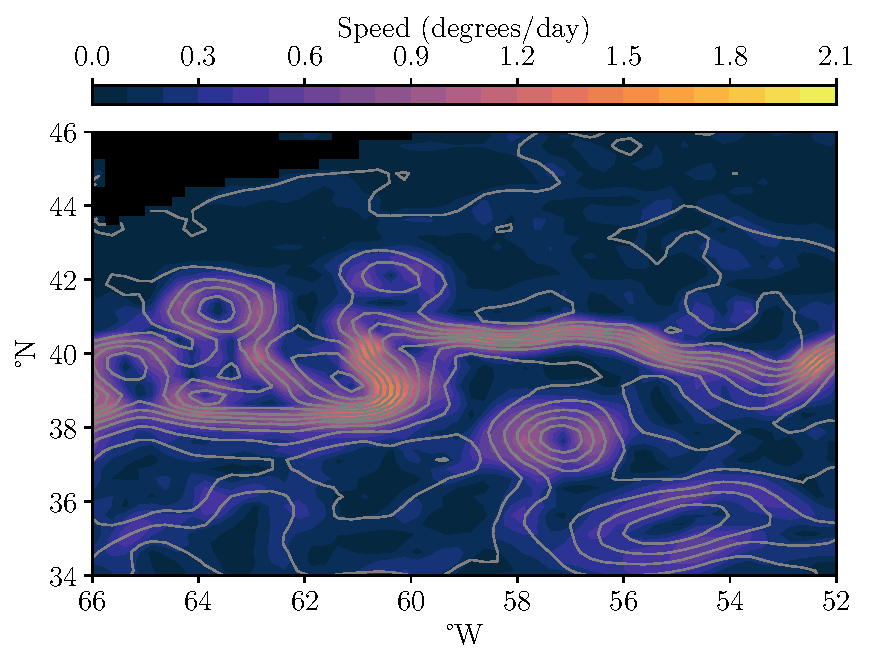
\includegraphics[width=\textwidth]{chp06_applications/figures/gulf_stream/streamlines_0}
% 			\caption{\(t = 0\) (midnight \DTMdisplaydate{2020}{01}{01}{})}
% 		\end{subfigure}
% 		\begin{subfigure}{0.49\textwidth}
% 			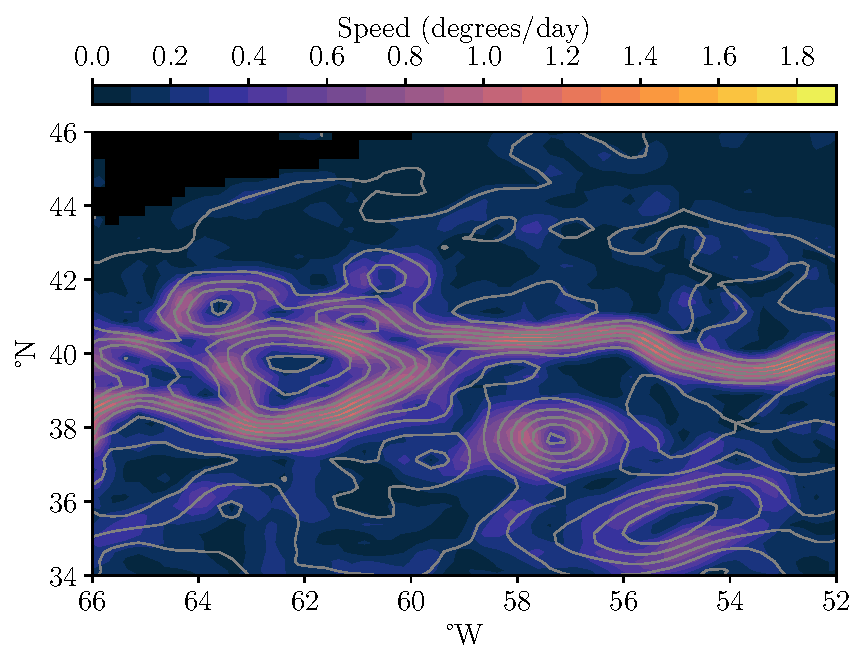
\includegraphics[width=\textwidth]{chp06_applications/figures/gulf_stream/streamlines_5}
% 			\caption{\(t = 5\) (midnight \DTMdisplaydate{2020}{01}{6}{})}
% 		\end{subfigure}
% 		\begin{subfigure}{0.49\textwidth}
% 			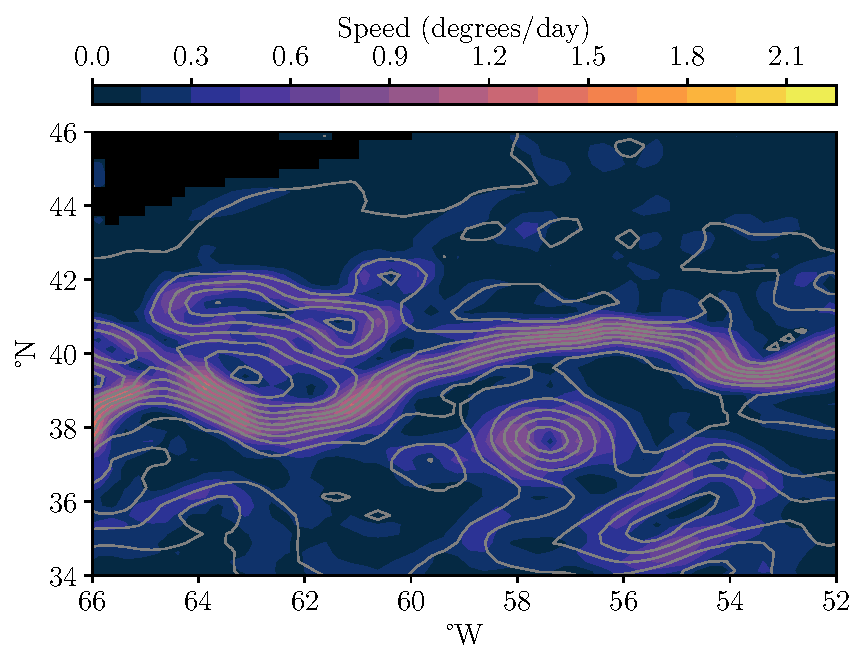
\includegraphics[width=\textwidth]{chp06_applications/figures/gulf_stream/streamlines_10}
% 			\caption{\(t = 10\) (midnight \DTMdisplaydate{2020}{01}{11}{})}
% 		\end{subfigure}
% 		\begin{subfigure}{0.49\textwidth}
% 			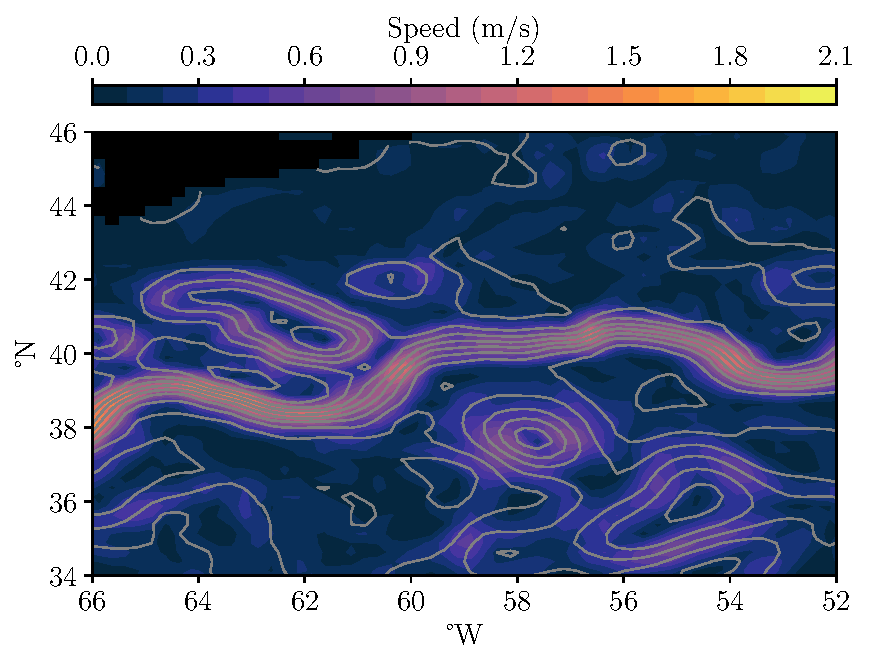
\includegraphics[width=\textwidth]{chp06_applications/figures/gulf_stream/streamlines_15}
% 			\caption{\(t = 15\) (midnight \DTMdisplaydate{2020}{01}{16}{})}
% 		\end{subfigure}
% 		\caption{The absolute surface current speed (coloured) and contours of the sea-surface height (streamlines of the flow, in grey) of the Gulf Stream dataset, at various times chosen to demonstrate the formation and separation of an eddy from the stream.
% 			The black region indicates missing data, due to the presence of land.
% 			All times are in Greenwich Mean Time.}
% 		\label{fig:na_motive_flow}
% 	\end{center}
% \end{figure}

\begin{figure}
	\centering
	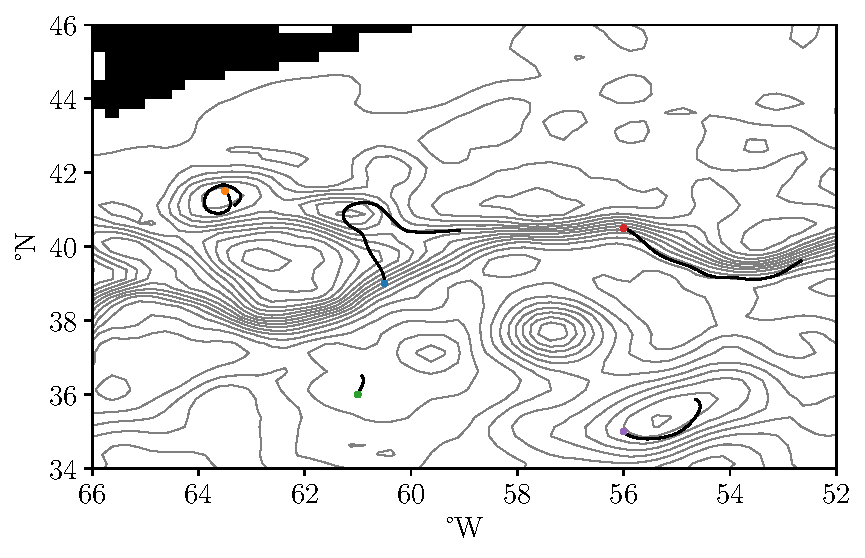
\includegraphics[width=\textwidth]{chp06_applications/figures/gulf_stream/det_trajs}
	\caption{Several trajectories (in heavy black) that solve \cref{eqn:natl_ode} and describe the motion of drifters on the surface of the Gulf Stream.
		Each trajectory is initialised at a coloured point at \(t = 0\) (midnight \DTMdisplaydate{2020}{1}{1}{}), and evolved by numerically solving \cref{eqn:natl_ode} up to midnight \(t = 7\) (midnight \DTMdisplaydate{2020}{1}{8}{}).
		Instantaneous streamlines at the final time \(t = 7\) are displayed in grey.}
	\label{fig:natl_ode_sols}
\end{figure}

The velocity data is Eulerian and unsteady (varying with time), so to predict the position of a drifter we must solve for a Lagrangian trajectory.
This requires interpolating the velocity data between the spatial and temporal gridpoints, for which we use a linear interpolate.
Let
\[
	x_t = \left(x_t^{(\mathrm{lon})}, x_t^{(\mathrm{lat})}\right)^{\T}
\]
denote the longitudinal (in degrees east) and latitudinal (in degrees north) position of the drifter \(t\) days after midnight \DTMdisplaydate{2020}{01}{01}{-1}.
The deterministic model for \(x_t\), constructed purely from the interpolated velocity data, is
\begin{equation}\label{eqn:natl_ode}
	\dod{}{t}\begin{bmatrix}
		x_t^{(\text{lon})} \\ x_t^{(\text{lat})}
	\end{bmatrix} = \begin{bmatrix}
		\tilde{u}\!\left(x^{(\mathrm{lon})}_t, x^{(\mathrm{lat})}_t, t\right) \\ \tilde{v}\!\left(x^{(\mathrm{lon})}_t, x^{(\mathrm{lat})}_t, t\right)
	\end{bmatrix},
\end{equation}
where \(\tilde{u}\) and \(\tilde{v}\) are the interpolated zonal and meridional velocities respectively.
\Cref{fig:natl_ode_sols} shows some example trajectories that solve \cref{eqn:natl_ode}, evolving over the span of a week.
Contours of the sea surface height at \(t = 7\) are also shown in grey, which corresponds to those of the instantaneous streamfunction and provides an indication of the flow structure.
The stream itself is fast-moving and a prominent feature of the flow, and drifters starting within the stream (i.e.\ the blue and red points) are accordingly transported along it.
Along the stream, eddies form and break off (roughly indicated by the circular regions in the sea-surface height contour map), and trajectories that start within an eddy (i.e.\ orange and purple points) typically remain there.
Away from the stream and the eddies, the flow is relatively isotropic and slow-moving, resulting in the short and unremarkable trajectory starting from the green point.

\begin{figure}
	\centering
	\begin{subfigure}{0.49\textwidth}
		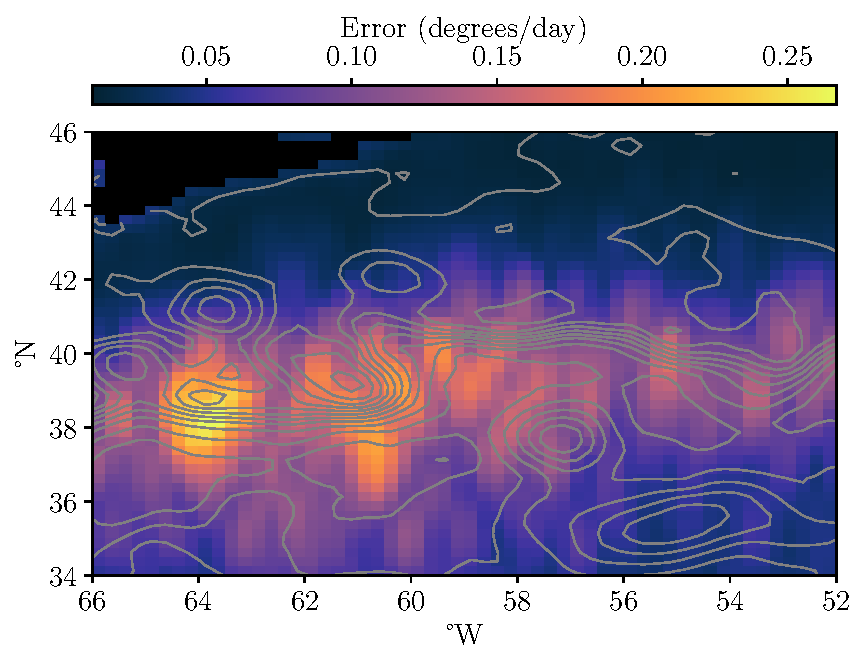
\includegraphics[width=\textwidth]{chp06_applications/figures/gulf_stream/u_err_0}
		\caption{Zonal component}
	\end{subfigure}
	\begin{subfigure}{0.49\textwidth}
		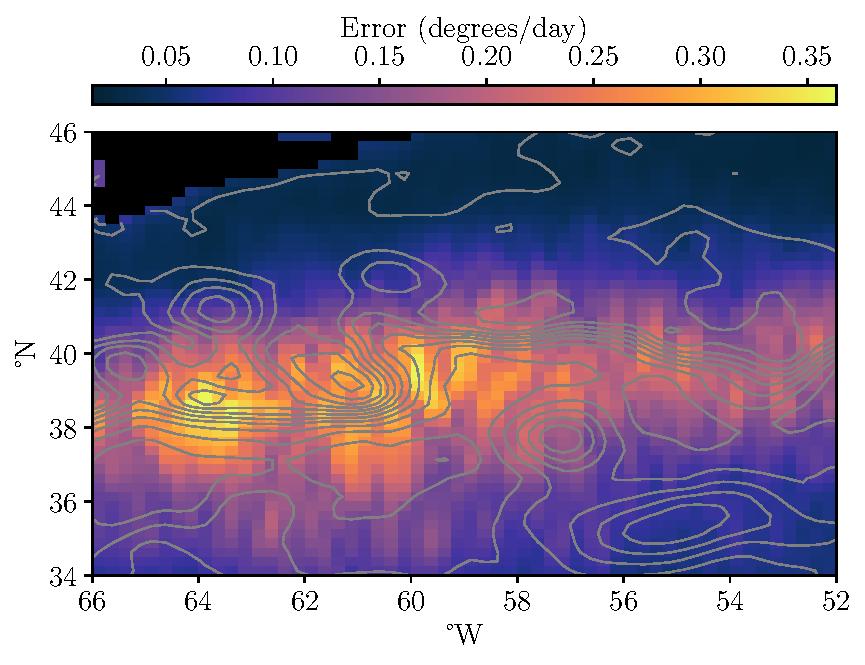
\includegraphics[width=\textwidth]{chp06_applications/figures/gulf_stream/v_err_0}
		\caption{Meridional component}
	\end{subfigure}
	\caption{The mapping error in the (a) zonal (longitudinal) and (b) meridional (latitudinal) velocity components at midnight \DTMdisplaydate{2020}{01}{01}{-1} (\(t = 0\)).}
	\label{fig:natl_err}
\end{figure}

We may think of \cref{eqn:natl_ode} as our ``best available'' deterministic model for the time evolution of the drifter position; if the data (and the subsequent interpolation) were correct, then \cref{eqn:natl_ode} would provide accurate predictions.
However, this is certainly not the case and there are many sources of uncertainty not accounted for by \cref{eqn:natl_ode}, including measurement error and the unresolved flow behaviour between gridpoints.
The dataset additionally includes estimates for the mapping error (an estimate of the variance) in the zonal and meridional velocity measurements, which indicates measurement error. %; typically the error is smaller in regions directly under satellite tracks.
The mapping error in each velocity component at \(t = 0\) is shown in \Cref{fig:natl_err}, as an example of the structure of the field, along with contours of the sea surface height.
The error varies with time but retains the main structure where it is largest along the Gulf Stream and features a stratified appearance because satellite measurements are more accurate directly under the tracks followed by the instruments, which is not unexpected as this region contains the most complicated part of the flow.
We can capture the spatial and temporal variation in this mapping error by adding multiplicative noise to the deterministic model \cref{eqn:natl_ode}.
We use the following stochastic model:
\begin{equation}
	\dif \begin{bmatrix}
		x^{(\mathrm{lon})}_t \\ x^{(\mathrm{lat})}_t
	\end{bmatrix} = \begin{multlined}[t]
		\begin{bmatrix} \tilde{u}\!\left(x^{(\mathrm{lon})}_t, x^{(\mathrm{lat})}_t, t\right) \\ \tilde{v}\!\left(x^{(\mathrm{lon})}_t, x^{(\mathrm{lat})}_t, t\right) \end{bmatrix}\dif t \\
		+ \sqrt{L_r}\begin{bmatrix}
			\sqrt{\tilde{u}_{\mathrm{err}}\!\left(x^{(\mathrm{lon})}_t, x^{(\mathrm{lat})}_t, t\right)} & 0                                                                                           \\
			0                                                                                           & \sqrt{\tilde{v}_{\mathrm{err}}\!\left(x^{(\mathrm{lon})}_t, x^{(\mathrm{lat})}_t, t\right)}
		\end{bmatrix} \dif W_t,
	\end{multlined}
	\label{eqn:natl_sde}
\end{equation}
where \(\tilde{u}_{\mathrm{err}}\) and \(\tilde{v}_{\mathrm{err}}\) are the linearly interpolated error estimates for the zonal and meridional velocities (converted to degrees per day using the same transformation \cref{eqn:natl_vel_conv} as was done on the velocity data), and \(L_r = 0.25^\circ\) is the spatial resolution of the data.
Our choice for the diffusion matrix \(\sigma\) comes from the intuition that \(L_r\sigma\sigma^{\T}\) represents the instantaneous variance of the noise in our stochastic differential equation and to ensure that the units in \cref{eqn:natl_sde} are consistent with the convention that \(\dif W_t \sim \sqrt{\mathrm{days}}\) \citep{Oksendal_2003_StochasticDifferentialEquations}.
Both coefficients depend on time and the noise is multiplicative, making \cref{eqn:natl_sde} the most general type of SDE that our theory is equipped to handle.
In the framework of \Cref{ch:linear_theory}, the noise scale is \(\epsilon = \sqrt{L_r} = \sqrt{0.25^\circ}\) and we treat this value as being fixed by the data and model.
The introduction of noise in \cref{eqn:natl_sde} can improve over \cref{eqn:natl_ode} by accounting for both the data-informed measurement error and unresolved behaviours between gridpoints, in the fashion of stochastic parameterisation.
This is, however, only one choice for such a model; the following analysis could be applied to a better-informed stochastic model.




% The derivatives \(\nabla u\) of the deterministic velocity field in \cref{eqn:natl_sde} are approximated via the centred finite-differences,
% \begin{align*}
% 	\dpd{u\left({x^{(\text{lon})}}, {x^{(\text{lat})}}, t\right)}{{x^{(\text{lon})}}} & \approx \frac{u\left(x^{(\text{lon})} + L_r, x^{(\text{lat})}, t\right) - u\left(x^{(\text{lon})} - L_r, x^{(\text{lat})}, t\right)}{2 L_r},
% \end{align*}
% and similar for the remaining derivatives.



% We will now introduce an example of a differential equation model constructed from observed data, which we will use throughout this chaper, and explore further in \Cref{ch:appls}.
% In particular, the technical details of this example will be provided in \Cref{sec:appl_ocean}.

% Suppose we are interested in tracking the position of a drifter on the surface of the Gulf Stream.
% The only information we have available are measurements of the eastwards (zonal) and northwards (meridional) velocities at the surface, derived from altimetry (sea surface height) data.
% Such data is available from the European Commission`s Copernicus Marine Environment Monitoring Service.

% For the purposes of this example, assume that the position of the drifter at the initial time is known exactly\footnote{In practice, of course, this will not be the case, but this will introduce even more uncertainty into our model, furthering reinforcing the purpose of this example.}.
% Assuming that the interpolated data provided an accurate model of the sea surface velocity, the position \(x_t\) of the drifter on the surface at time \(t\) is the solution to the ordinary differential equation
% \begin{equation}\label{eqn:na_motiv_ode}
% 	\dod{x_t}{t} = u\left(x_t, t\right),
% \end{equation}
% subject to the known initial position \(x_0\), where \(u\) is the appropriately interpolated surface velocity data.
% To illustrate the time-varying dynamics of the Stream, \Cref{fig:na_motiv_flow} plots contours the sea-surface height, which correspond to the time-varying streamfunction of the flow, and therefore solutions to \cref{eqn:na_motiv_ode}, at various times.
% An important feature of the flow is that there are significantly different qualitative regimes; there is the rapidly moving stream itself, the eddies that are shed and slow moving, and isotropic regions in between where the current is comparatively slow.



% We can easily solve \cref{eqn:na_motiv_ode} numerically to obtain a predicted position for our drifter on day \(t\).
% % We term \cref{eqn:na_motiv_ode} the \emph{deterministic model}, since given the data we have available, it serves as our best purely deterministic model for the position of the drifter.
% Suppose that our drifter begins within the stream itself, at \(x_0 = \left(-60.5, 39\right)^{\T}\), \Cref{fig:na_motiv_det} plots the resulting trajectory (in white) obtained by solving \cref{eqn:na_motiv_ode} numerically, over the span of 7 days starting from midnight \DTMdisplaydate{2020}{01}{01}{}.
% Based on this model, we expect that the drifter will follow the Stream, which can inform efforts to locate the drifter.

% \begin{figure}
% 	\begin{center}
% 		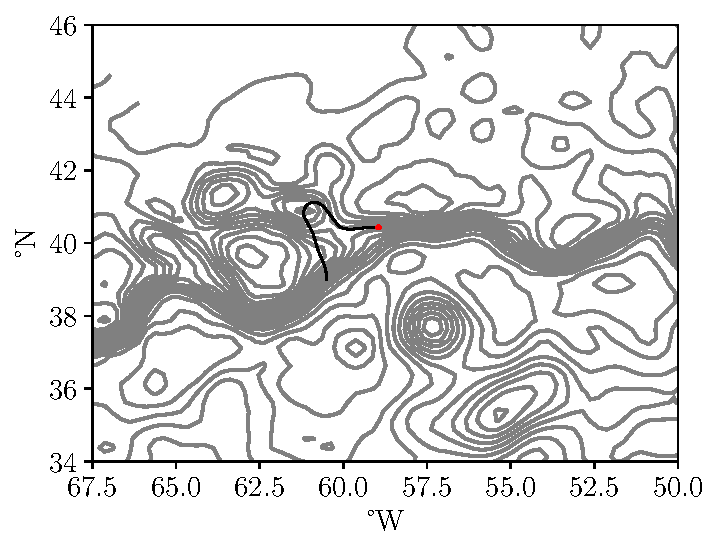
\includegraphics[width=\textwidth]{chp06_applications/figures/gulf_stream_motivation/det_traj.pdf}
% 		\caption{The time evolution of the solution (obtained by numerically integrating the velocity data) to the deterministic system corresponding to \cref{eqn:natl_sde}, from initial condition \(x_0 = \left(-60.5, 39\right)^{\T}\) from 01/01/2021 (\(t = 0\)) to 08/01/2021 (\(t = 8\)).
% 			Contours of the sea surface height at the final time \(t = 8\) are included in grey to indicate the position of the Gulf Stream and nearby eddies in the flow.}
% 		\label{fig:na_motiv_det}
% 	\end{center}
% \end{figure}

% To improve our predictions of the future position of the drifter, we should attempt to account for this uncertainty in our model \cref{eqn:na_motiv_ode}.
% The altimetry-derived data also includes measures of error in each component of the velocity at each spatiotemporal gridpoint, so we can use these measurements to model the ongoing observational error in \(u\).
% We can extend \cref{eqn:na_motiv_ode} as a stochastic differential equation, where the unresolved uncertainty is parameterised as a white-noise process scaled by measurement error.
% Specifically, we formulate the drifter position as \cref{eqn:natl_sde} in \Cref{sec:gulf_stream}, which is explained in more detail in that section.
% For our purposes here, \cref{eqn:natl_sde} is a stochastic differential equation analogy of \cref{eqn:natl_sde} that we can solve numerically to obtain approximate solution samples.

% \Cref{fig:na_motiv_rels} shows us the result of numerically solving a stochastic differential equation formulation (specifically ) of the Lagrangian trajectory model.
% This is a ``more correct'' model than the deterministic counterpart, in the sense that it is attempting to account for the unknowable measurement error and unresolved subgrid effects.
% Each realisation here could correspond to our drifter, and we see a far different picture than the deterministic model alone provided.
% Qualitatively, rather than following the Stream itself, a proportion of particles are caught in one of two eddies which have formed and broken off from the Stream.

% \begin{figure}
% 	\begin{center}
% 		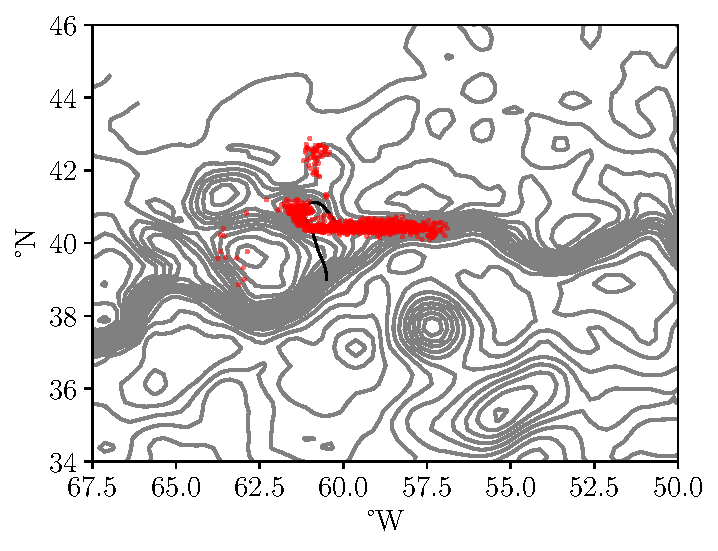
\includegraphics[width=\textwidth]{chp06_applications/figures/gulf_stream_motivation/num_rels.pdf}
% 		\caption{The same visualisation of the deterministic behaviour of the Gulf Stream example as \Cref{fig:na_motive_det}, but with the final positions of 10000 numerical realisations of a stochastic model, each indicated by a red point.}
% 		\label{fig:na_motiv_rels}
% 	\end{center}
% \end{figure}

% Although deterministic models are often easier to work with analytically and far more efficient to solve numerically, these models are limited.
% By explicitly accounting for uncertainty with a stochastic, we can expand the scope of our model and provide more realistic and useful predictions, at the cost of a more complicated model.
% This idea of introducing stochastic components into a deterministic model to account for unresolved and unknown aspects has been used extensively in recent times across scientific applications, notably atmospheric, climate, and oceanographic modelling.
% We provide an overview of this so-called stochastic parameterisation in the next section, and highlight how the work of this thesis fits in with the needs of that field.

\section{Stochastic sensitivity}
We first compute the stochastic sensitivity field to evaluate the impact of uncertainty (formulated by the SDE \cref{eqn:natl_sde}) on the predictions of the deterministic model \cref{eqn:natl_ode}.
As in \Cref{sec:comput_s2}, this example demonstrates the computation of stochastic sensitivity from the covariance matrix, rather than provide any new insight.
\citet{BadzaEtAl_2023_HowSensitiveAre} provide a similar example of computing the stochastic sensitivity field for a similar sea-surface dataset of the Gulf Stream, albeit using the original method of calculation \citep{Balasuriya_2020_StochasticSensitivityComputable}.

\begin{figure}
	\centering
	\begin{subfigure}{\textwidth}
		\includegraphics[width=0.49\textwidth]{chp06_applications/figures/gulf_stream/S2_field_grid}
		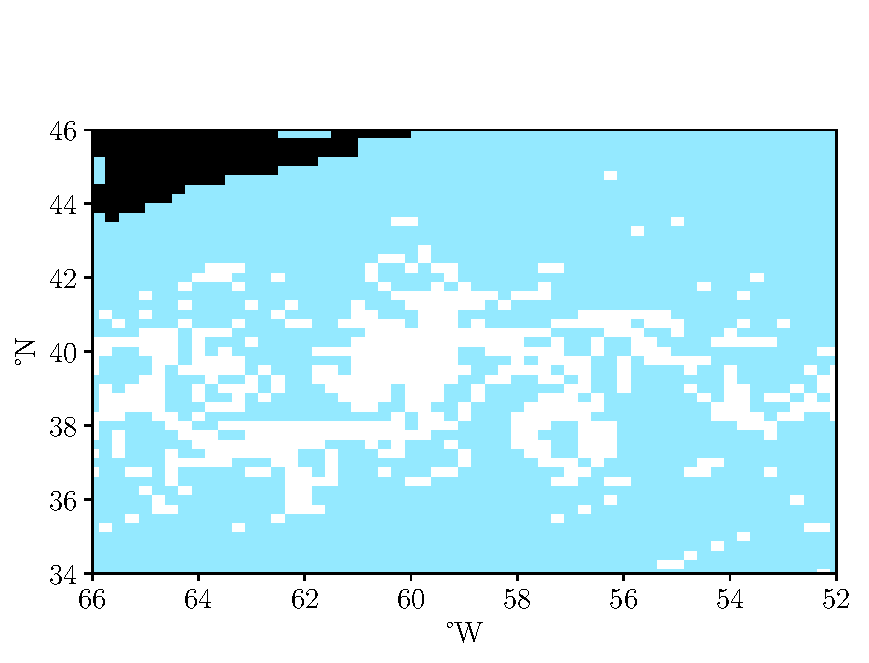
\includegraphics[width=0.49\textwidth]{chp06_applications/figures/gulf_stream/S2_robust_grid_2.0}
		\caption{At the \(0.25^\circ \times 0.25^\circ\) resolution of the velocity data.}
		\label{fig:na_s2_grid}
	\end{subfigure}
	\begin{subfigure}{\textwidth}
		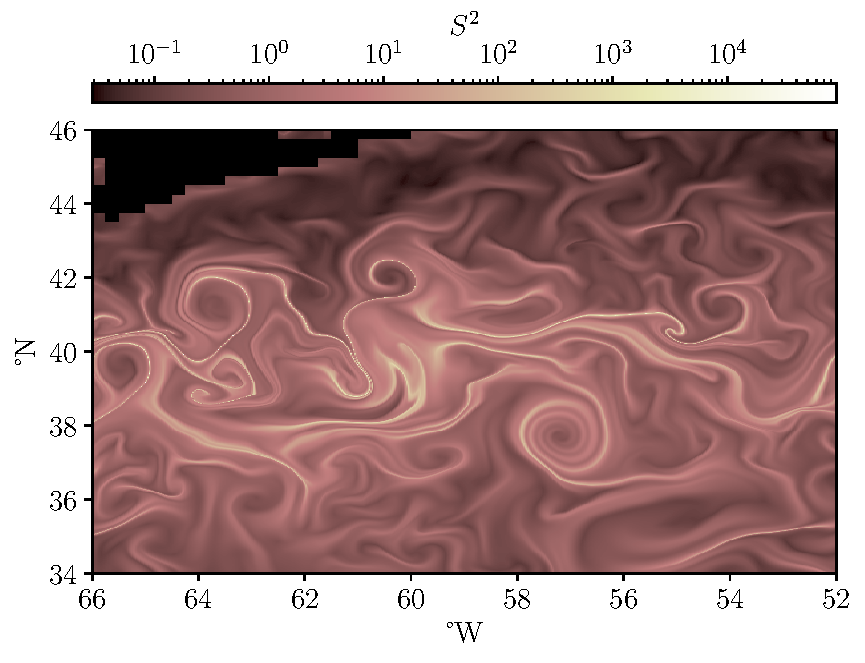
\includegraphics[width=0.49\textwidth]{chp06_applications/figures/gulf_stream/S2_field_high}
		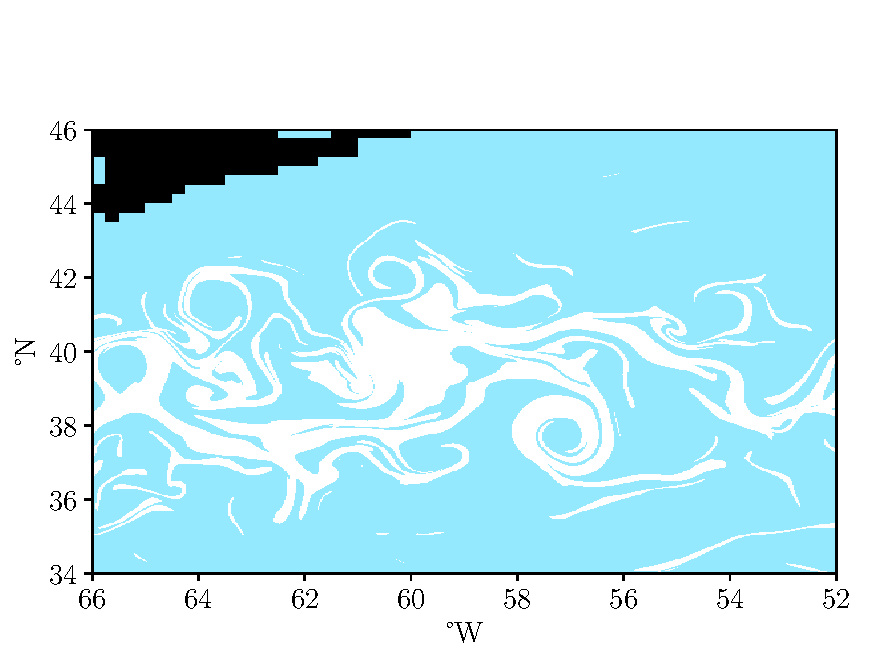
\includegraphics[width=0.49\textwidth]{chp06_applications/figures/gulf_stream/S2_robust_high_2.0}
		\caption{At the higher resolution of \(0.025^\circ \times 0.025^\circ\).}
		\label{fig:na_s2_high}
	\end{subfigure}
	\caption{(Left) The stochastic sensitivity fields computed from the linearisation covariance matrix on a grid of initial conditions, at two different resolutions.
		(Right) From each field, robust sets are extracted with a threshold of \(R = 2^\circ\) and shown in cyan.
	}
	\label{fig:na_s2}
\end{figure}

\Cref{fig:na_s2_grid} plots the stochastic sensitivity field for a grid of initial conditions at the \(0.25^\circ \times 0.25^\circ\) resolution of the velocity data, over the timespan of a week, from midnight \DTMdisplaydate{2020}{01}{01}{-1} (\(t = 0\)) to midnight \DTMdisplaydate{2020}{01}{08}{-1} (\(t = 7\)).
Each initial condition corresponds to a point at which the surface velocity data was available.
% The stochastic sensitivity field quantifies the magnitude of the uncertainty (modelled by the SDE \cref{eqn:natl_sde}) in the deterministic trajectory (solving \cref{eqn:natl_ode}) starting from each initial condition.
Although the resolution of the velocity data is low, we can still distinguish the stream itself as a region of high uncertainty.
Away from the stream (either north or south of it), the flow is reasonably isotropic and the level of noise from measurement error is small, so there are relatively small \(S^2\) values.
The \(S^2\) field also highlights an eddy-like structure, centred around \(57^\circ\)W and \(38^\circ\)N, with a larger uncertainty on the boundary and a smaller within.

\citet{Balasuriya_2020_StochasticSensitivityComputable} provided a simple method for extracting possibly coherent sets from the stochastic sensitivity field, by taking the initial conditions for which the \(S^2\) value is under a certain threshold.
Using a threshold of \(R = 2^\circ\), the right-hand side of \Cref{fig:na_s2_grid} shows in cyan the initial conditions which correspond to a robust set.
% Additional plots showing robust sets extracted with different thresholds are provided in \Cref{app:s2_robust}.
We see that the regions away from the stream emerge as robust sets.
These sets do not include parts of the stream, because of the larger uncertainty.
However, the low resolution of the data means we cannot make any further conclusions, as the finer structure is unresolved.

The resolution of the data is a significant limitation of the deterministic model; since the velocity data has been interpolated between gridpoints, any conclusions relying on the deterministic model alone cannot be trusted at higher resolutions.
% For instance, if we were to compute the finite-time Lyapunov exponent of \cref{eqn:natl_ode} on a set of ini
Although the stochastic model also uses this interpolated data, the model is in some sense accounting for the uncertainty introduced by the interpolation.
We are resolving the behaviour of the system between the gridpoints by introducing stochastic noise.
Since stochastic sensitivity is a property of the \emph{stochastic} system and not just the deterministic one, we are permitted to investigate and make conclusions from this field at a higher resolution than that prescribed by the data.
This is an advantage of stochastic sensitivity over other deterministic measures, such as the finite-time Lyapunov exponent, which do not account for unresolved effects.
\Cref{fig:na_s2_high} show the stochastic sensitivity field computed on a \(0.025^\circ\times 0.025\) grid of initial conditions, at a higher resolution than the velocity data.
We see several eddy-like structures highlighted above and below the stream, where uncertainty is large on the boundaries of the eddies and smaller within.
These eddies were not all apparent in the lower-resolution \(S^2\) field or in the corresponding robust sets.
% The stream is outlined by regions of high uncertainty, which is expected as near these edges trajectories can undergo qualitatively very different behaviours by either remaining in the stream or leaving it in an eddy.
% On the right-hand side of \Cref{fig:na_s2_high}, we show robust sets extracted from the higher resolution stochastic sensitivity field, again using a threshold of \(2^\circ\).
The complicated structure of the stream is better resolved in the higher-resolution field and emerges as regions of non-robustness (that is, not contained in the robust sets).
The centres of the eddies, where we expect coherency in the deterministic system, are also included in the robust set.
By increasing the resolution, we can therefore identify regions of low uncertainty and distinguish finer structures within the flow.
% \td{Conclude by summarising the implications of stochastic sensitivity - what have we just done?}





% \begin{figure}
% 	\begin{center}
% 		\begin{subfigure}[t]{\textwidth}
% 			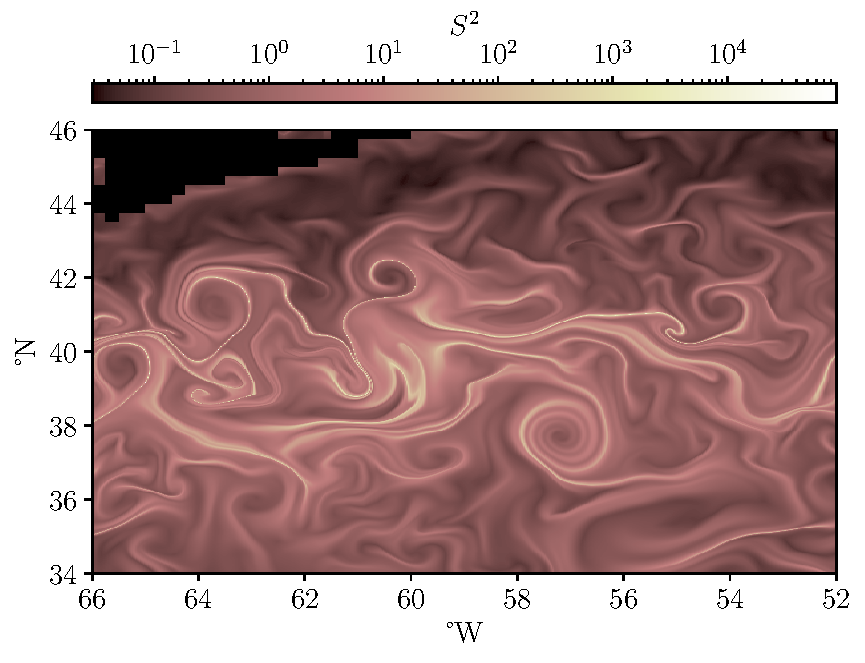
\includegraphics[width=\textwidth]{chp06_applications/figures/gulf_stream/S2_field_high}
% 			\caption{The stochastic sensitivity \(S^2\).}
% 		\end{subfigure}
% 		% \begin{subfigure}[t]{0.49\textwidth}
% 		% 	\includegraphics[width=\textwidth]{chp06_applications/figures/gulf_stream/s2_field_high}
% 		% 	\caption{The minimum eigenvalue of the covariance matrix.}
% 		% \end{subfigure}
% 		% \begin{subfigure}[t]{0.49\textwidth}
% 		% 	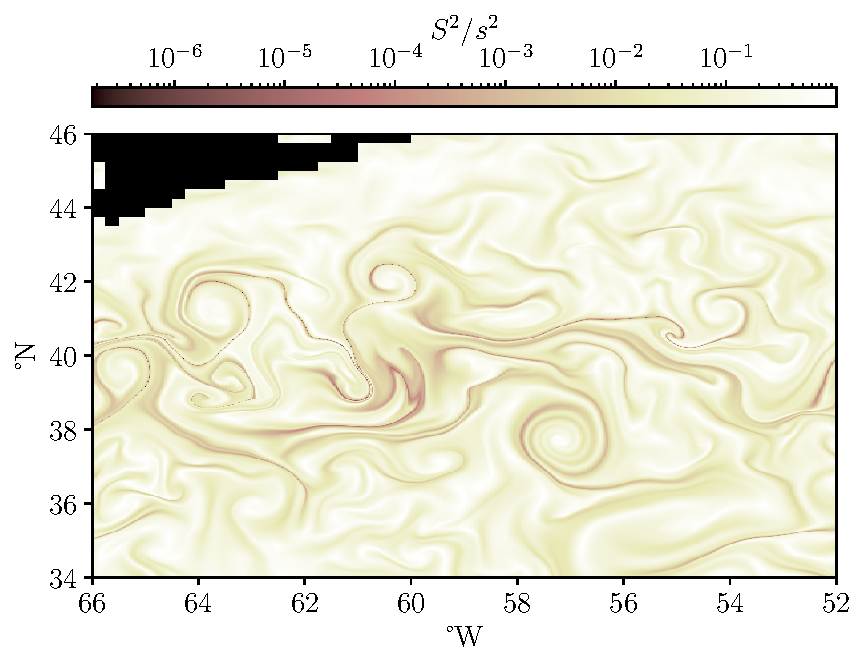
\includegraphics[width=\textwidth]{chp06_applications/figures/gulf_stream/ratio_field_high}
% 		% 	\caption{The ratio of the stochastic sensitivity value (maximum eigenvalue) and the minimum eigenvalue of the covariance matrix, which captures the `narrowness' of the linearised distribution.}
% 		% \end{subfigure}
% 		% \begin{subfigure}[t]{0.49\textwidth}
% 		% 	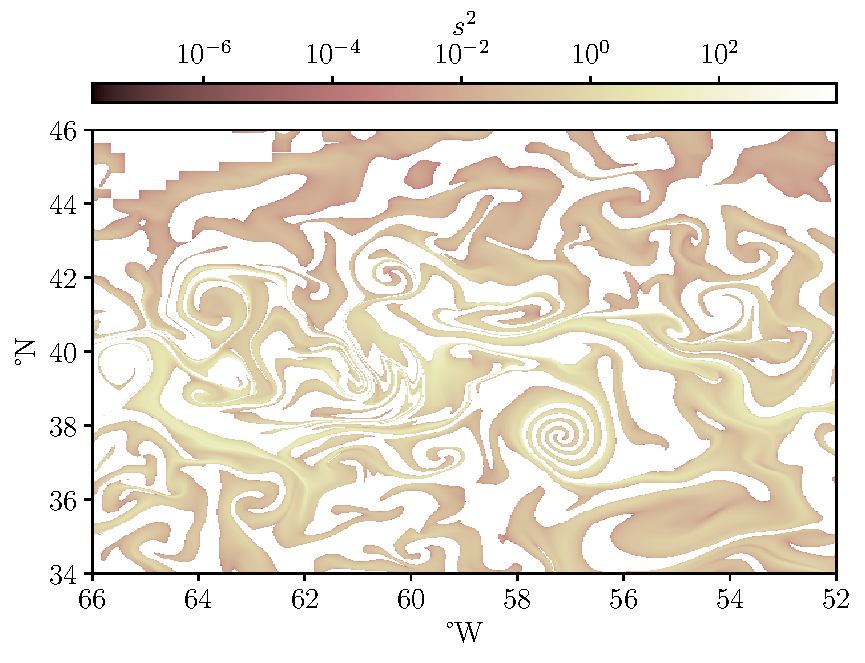
\includegraphics[width=\textwidth]{chp06_applications/figures/gulf_stream/cov_field_high}
% 		% 	\caption{The \((1,2)\)th entry of the covariance matrix, corresponding to the covariance between coordinates.
% 		% 		White indicates regions in which the entry is zero.}
% 		% \end{subfigure}
% 		\caption{Fields computed from the linearisation covariance matrix on a grid of initial conditions, in the same arrangement as \Cref{fig:na_s2} but at a higher resolution of \(0.025^\circ \times 0.025^\circ\).
% 			Note that values near the boundaries of the data and the land are not trustworthy, as the Gaussian approximations do not account for these boundaries.}
% 		\label{fig:na_s2_high}
% 	\end{center}
% \end{figure}



\section{Exploring a single trajectory}\label{sec:na_single}

\begin{figure}
	\begin{center}
		\begin{subfigure}[t]{0.7\textwidth}
			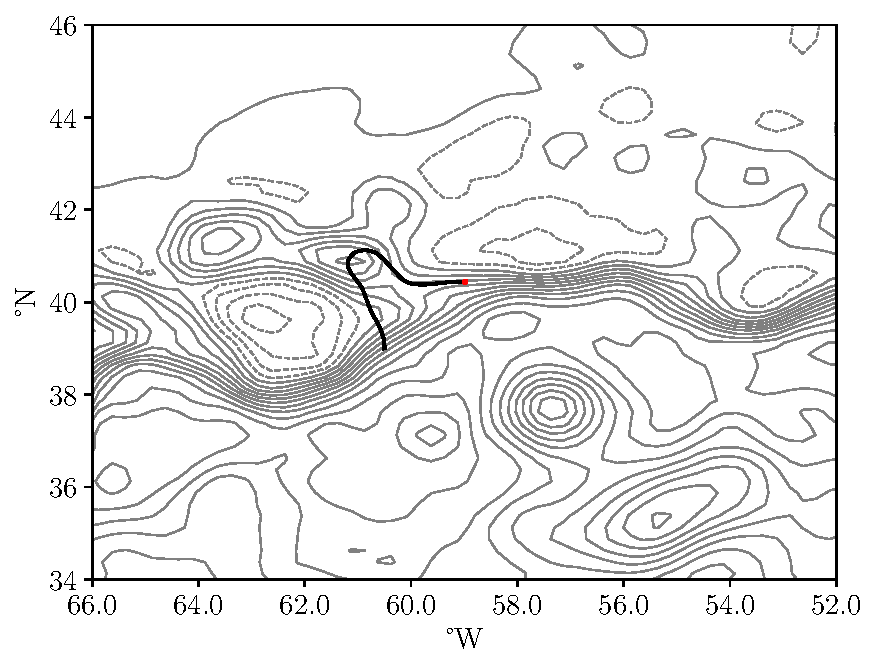
\includegraphics[width=\textwidth]{chp06_applications/figures/gulf_stream/det_traj.pdf}
			\caption{The solution to the deterministic model \cref{eqn:natl_ode}.}
			\label{fig:natl_det_traj}
		\end{subfigure}
		\begin{subfigure}[t]{0.7\textwidth}
			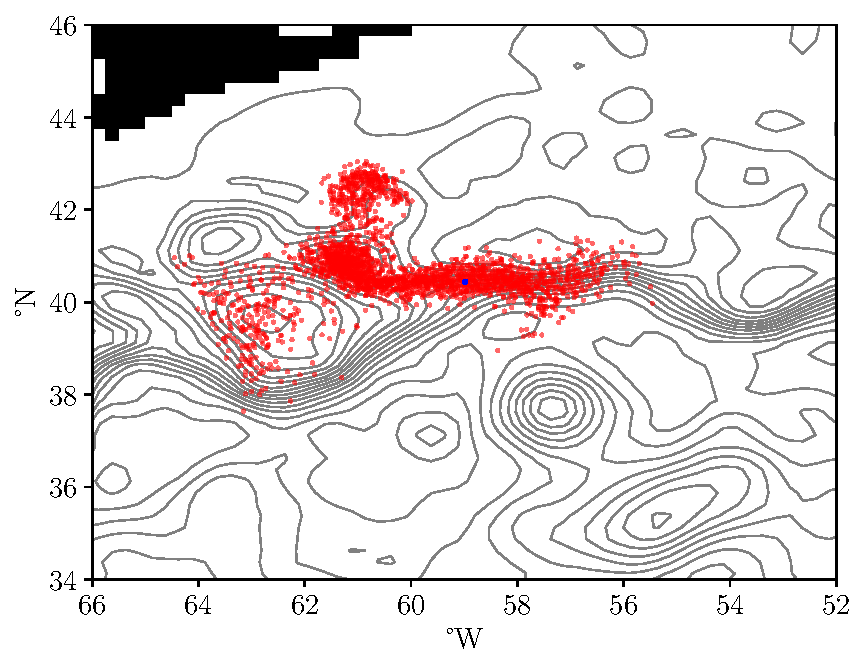
\includegraphics[width=\textwidth]{chp06_applications/figures/gulf_stream/traj_stoch_rels}
			\caption{Realisations of the solution to the stochastic model \cref{eqn:natl_sde}.}
			\label{fig:natl_stoch_rels}
		\end{subfigure}
		\caption{Solutions to the (a) deterministic model \cref{eqn:natl_ode} and (b) stochastic model \cref{eqn:natl_sde} for fixed initial condition \((-60.5, 39)^{\T}\) from midnight \DTMdisplaydate{2021}{01}{01}{-1} (\(t = 0\)) to midnight \DTMdisplaydate{2021}{01}{08}{-1} (\(t = 7\)), corresponding to a drifter on the surface of the Gulf Stream.
			The deterministic prediction at \(t = 7\) is indicated in blue in both figures, with the time evolution of the deterministic trajectory in black in (a).
			In (b), each red point corresponds to one of 2500 EM realisations of the stochastic solution at midnight \DTMdisplaydate{2021}{01}{08}{-1}.
			Contours of the sea surface height at \(t = 7\) are included in grey.}
	\end{center}
\end{figure}


We now focus our attention on a fixed initial condition for the drifter. % and explore the time-evolution of the resulting probability distribution arising from \cref{eqn:natl_sde}, to which we can apply the tools we have developed in \Cref{ch:linear_theory,ch:gmm}.
Suppose that, at midnight \DTMdisplaydate{2021}{01}{01}{-1}, the drifter is located within the stream at longitude \(60.5^\circ\)W and latitude \(39^\circ\)N.
We accordingly consider the evolution of the two models \cref{eqn:natl_ode} and \cref{eqn:natl_sde} with the initial condition \(x_0 = (-60.5, 39)^{\T}\).
By solving the deterministic model \cref{eqn:natl_ode} numerically, we predict the position of the drifter after \(t = 7\) days (at midnight \DTMdisplaydate{2021}{01}{08}{-1}) and show the time evolution of this solution trajectory in \Cref{fig:natl_det_traj}.
The jet stream transports the drifter.
This is the \emph{only} prediction of the deterministic model \cref{eqn:natl_ode}, but when accounting for uncertainty with the stochastic model \cref{eqn:natl_sde}, we get a more complicated picture.
\Cref{fig:natl_stoch_rels} shows the result of \(2500\) numerical realisations (obtained via Euler-Maruyama integration with a step size of \(1/24\) days) of the stochastic model \cref{eqn:natl_sde}, starting from the fixed initial condition \(x_0\) and evolved over the same week-long timeframe.
Each red point corresponds to a single realisation of the stochastic solution at midnight \DTMdisplaydate{2021}{01}{08}{-1} (\(t = 7\)).
Although many of the realisations are transported along the stream, many break off in eddies, resulting in several clusters of realisations.
Thus, with uncertainty in the model, the drifter may end up following distinctly different qualitative behaviour.
This example highlights the importance of stochastic models; the deterministic model provides a single prediction, but the dynamic behaviour of the flow means that any uncertainty can lead to vastly different predictions of the future state of the system.

\begin{figure}
	\centering
	% \begin{subfigure}{0.49\textwidth}
	% 	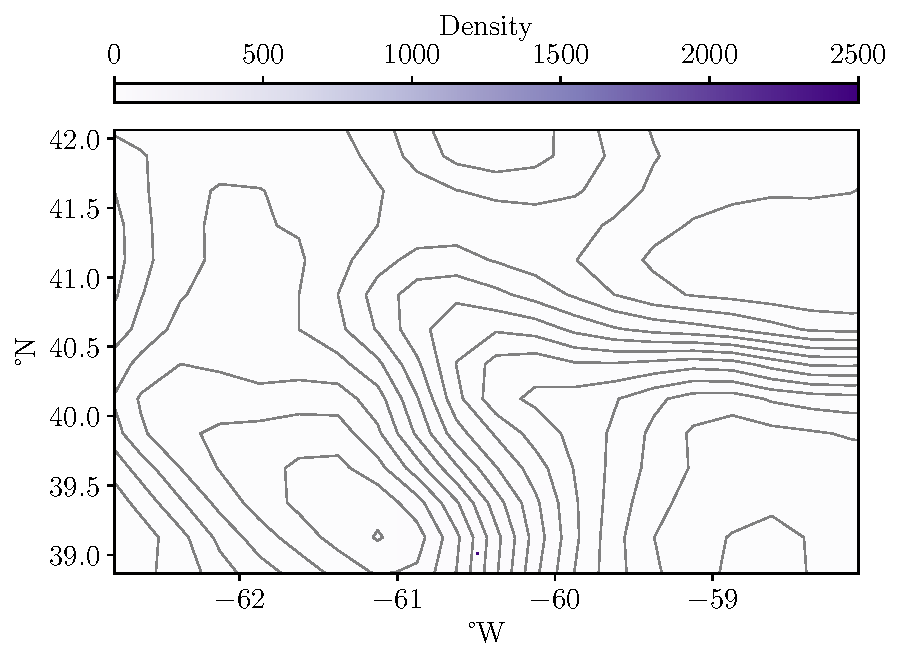
\includegraphics[width=\textwidth]{chp06_applications/figures/gulf_stream/rels_ssh_0.0}
	% 	\caption{Midnight \DTMdisplaydate{2021}{01}{01}{-1} (\(t = 0\)).}
	% 	\label{fig:na_hist_t3_0}
	% \end{subfigure}
	\begin{subfigure}{0.49\textwidth}
		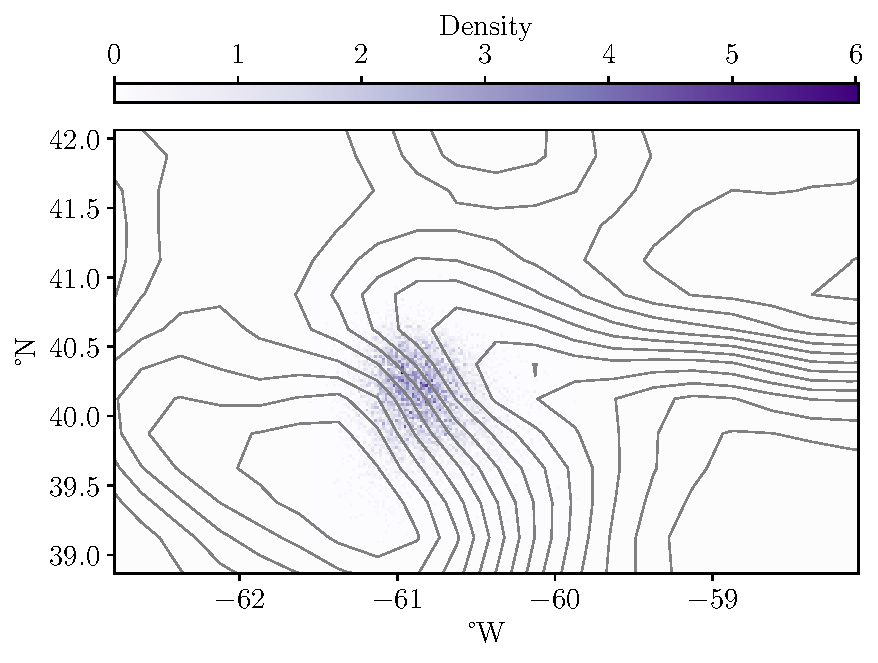
\includegraphics[width=\textwidth]{chp06_applications/figures/gulf_stream/rels_ssh_1.0}
		\caption{Midnight \DTMdisplaydate{2021}{01}{02}{-1} (\(t = 1\)).}
		\label{fig:na_hist_t3_1}
	\end{subfigure}
	\begin{subfigure}{0.49\textwidth}
		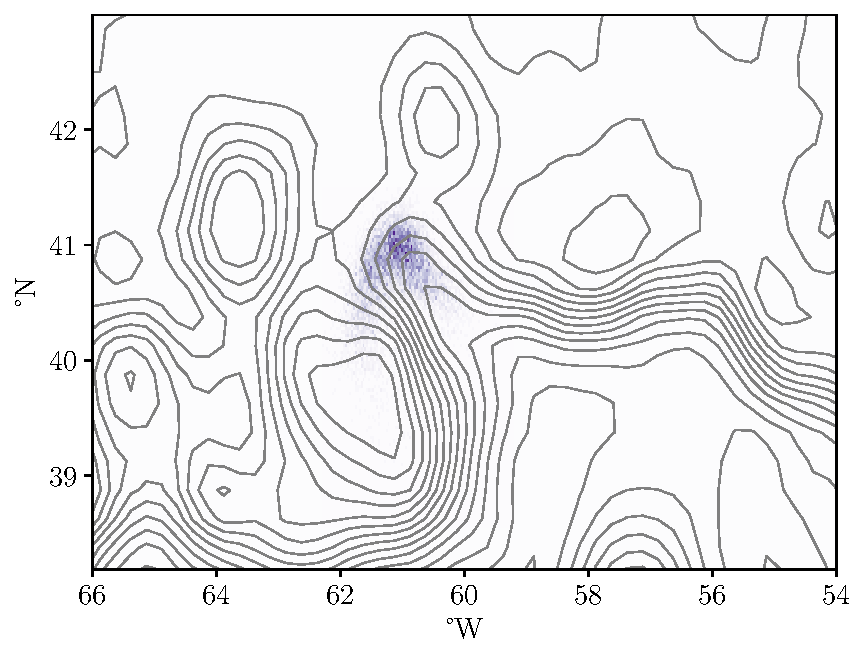
\includegraphics[width=\textwidth]{chp06_applications/figures/gulf_stream/rels_ssh_2.0}
		\caption{Midnight \DTMdisplaydate{2021}{01}{03}{-1} (\(t = 2\)).}
		\label{fig:na_hist_t3_2}
	\end{subfigure}
	\begin{subfigure}{0.49\textwidth}
		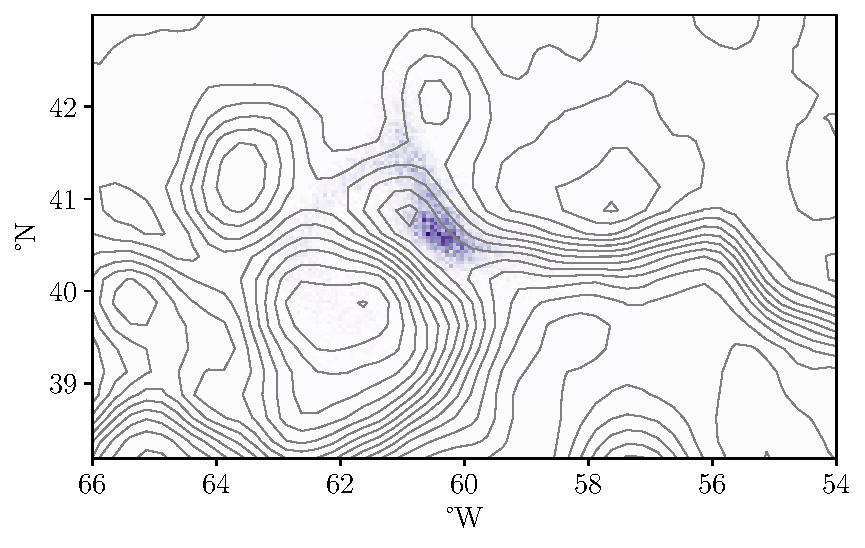
\includegraphics[width=\textwidth]{chp06_applications/figures/gulf_stream/rels_ssh_4.0}
		\caption{Midnight \DTMdisplaydate{2021}{01}{05}{-1} (\(t = 4\)).}
		\label{fig:na_hist_t3_3}
	\end{subfigure}
	\begin{subfigure}{0.49\textwidth}
		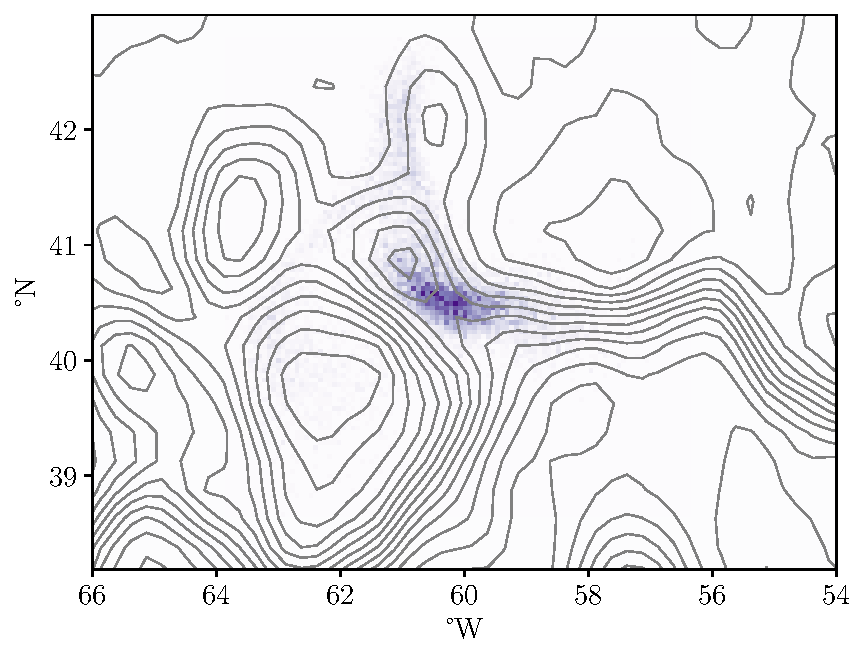
\includegraphics[width=\textwidth]{chp06_applications/figures/gulf_stream/rels_ssh_5.0}
		\caption{Midnight \DTMdisplaydate{2021}{01}{06}{-1} (\(t = 5\)).}
		\label{fig:na_hist_t3_4}
	\end{subfigure}
	\begin{subfigure}{0.49\textwidth}
		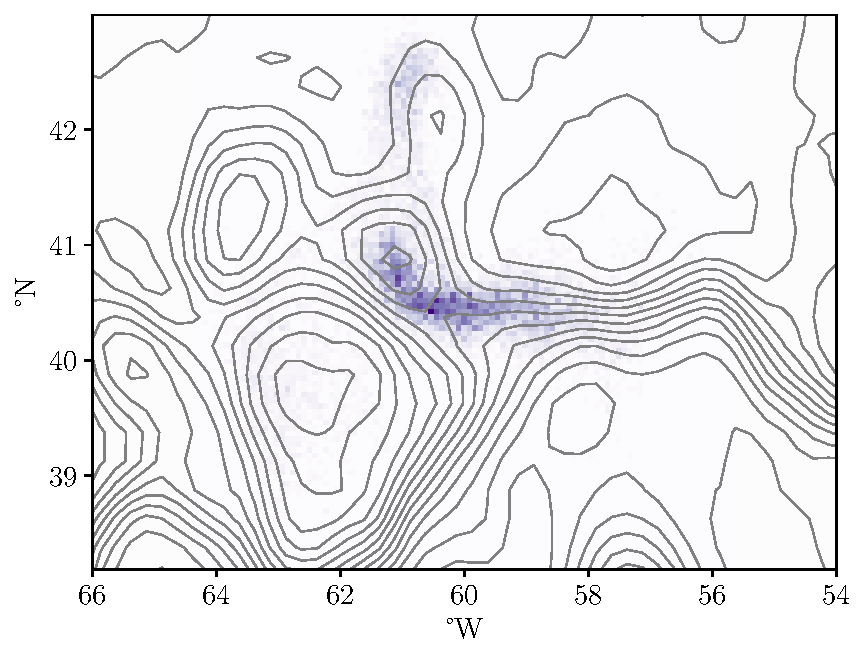
\includegraphics[width=\textwidth]{chp06_applications/figures/gulf_stream/rels_ssh_6.0}
		\caption{Midnight \DTMdisplaydate{2021}{01}{07}{-1} (\(t = 6\)).}
		\label{fig:na_hist_t3_5}
	\end{subfigure}
	\begin{subfigure}{0.49\textwidth}
		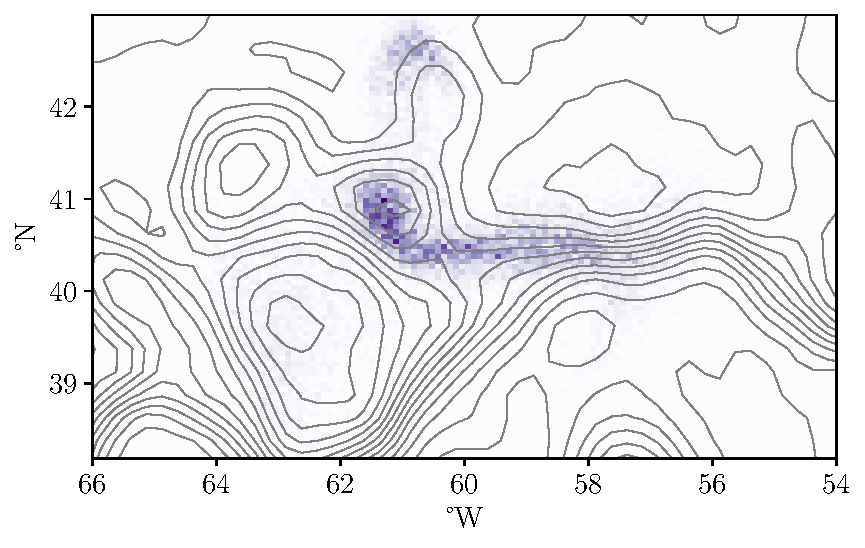
\includegraphics[width=\textwidth]{chp06_applications/figures/gulf_stream/rels_ssh_7.0}
		\caption{Midnight \DTMdisplaydate{2021}{01}{08}{-1} (\(t = 7\)).}
		\label{fig:na_hist_t3_6}
	\end{subfigure}
	\caption{Histograms representing the empirical distribution of the solution to \cref{eqn:natl_sde}, constructed from 10000 Euler-Maruyama samples, with darker colours indicating higher density.
		In grey are contours of the sea surface height which correspond to the instantaneous streamlines at time \(t\).}
	\label{fig:na_hist_t3}
\end{figure}


% We now move onto a more precise analysis of the time-evolution of the probability distribution of this solution to the stochastic model \cref{eqn:natl_sde}, and apply the tools we have developed in \Cref{ch:linear_theory,ch:gmm}.
To further understand the impact of the deterministic flow dynamics on the behaviour of the stochastic solution, \Cref{fig:na_hist_t3} plots the evolution, as histograms, of now 10000 EM samples up to midnight \DTMdisplaydate{2021}{01}{08}{-1} (\(t = 7\)).
The figure also includes contours of the sea surface height at each time to give some indication of the deterministic dynamics.
The stream propagates a majority of the stochastic realisations, but we see several trajectories leave the stream early and move westwards, creating an arc-like structure of smaller density in the empirical distribution.
A second cluster of realisations departs the stream starting around \(t = 4\) and moves northwards, likely due to the formation and break off of an eddy from the stream in the region.
The final distribution of realisations is therefore complicated, comprising numerous realisations that remained in the stream, a second cluster that is transported northwards by an eddy, and a small number that are scattered westwards.

\begin{figure}
	\begin{center}
		\begin{subfigure}{0.49\textwidth}
			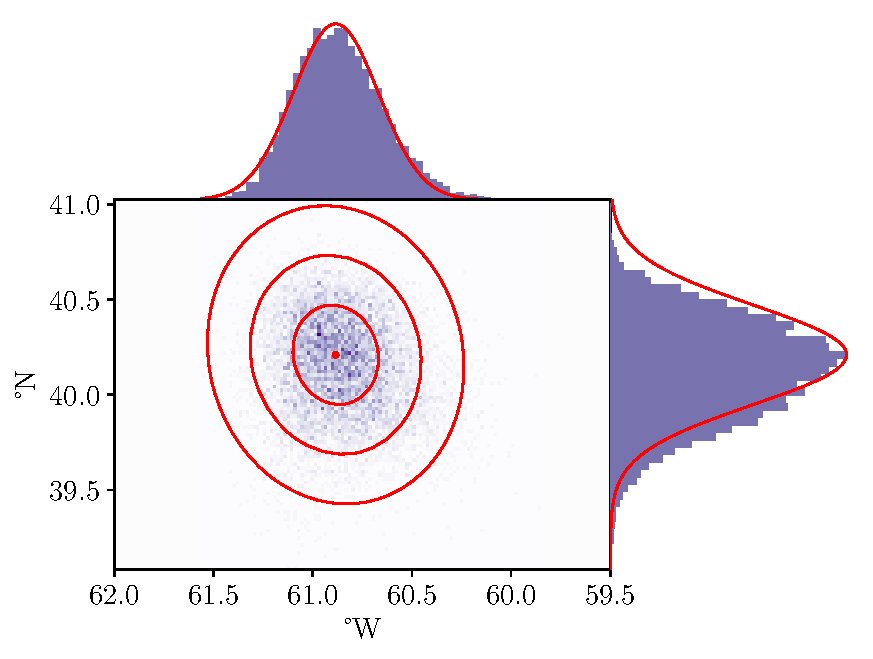
\includegraphics[width=\textwidth]{chp06_applications/figures/gulf_stream/traj_stoch_em_1.0}
			\caption{\(t = 1\) (midnight \DTMdisplaydate{2021}{01}{01}{-1})}
		\end{subfigure}
		\begin{subfigure}{0.49\textwidth}
			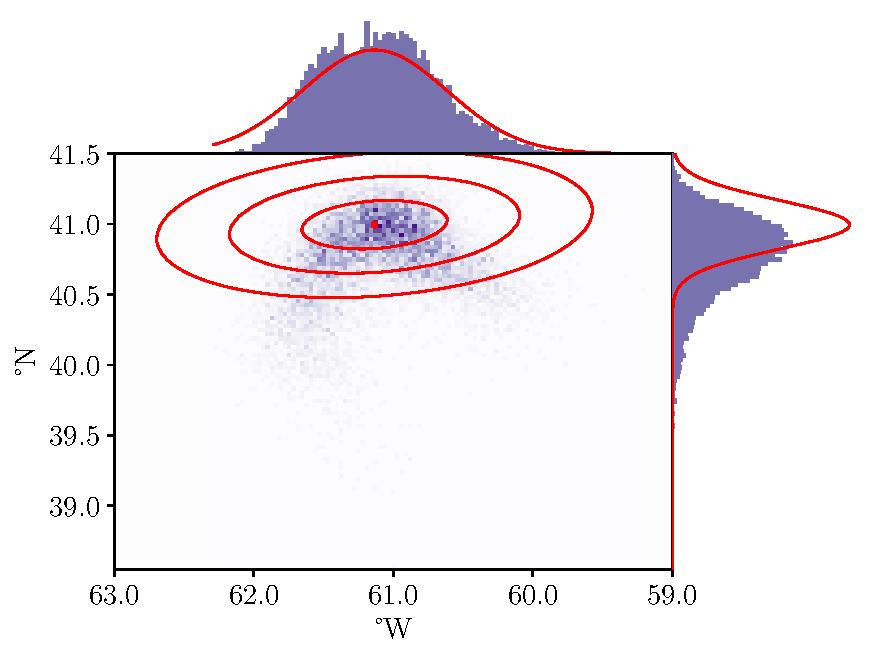
\includegraphics[width=\textwidth]{chp06_applications/figures/gulf_stream/traj_stoch_em_2.0}
			\caption{\(t = 2\) (midnight \DTMdisplaydate{2021}{01}{02}{-1})}
		\end{subfigure}
		\begin{subfigure}{0.49\textwidth}
			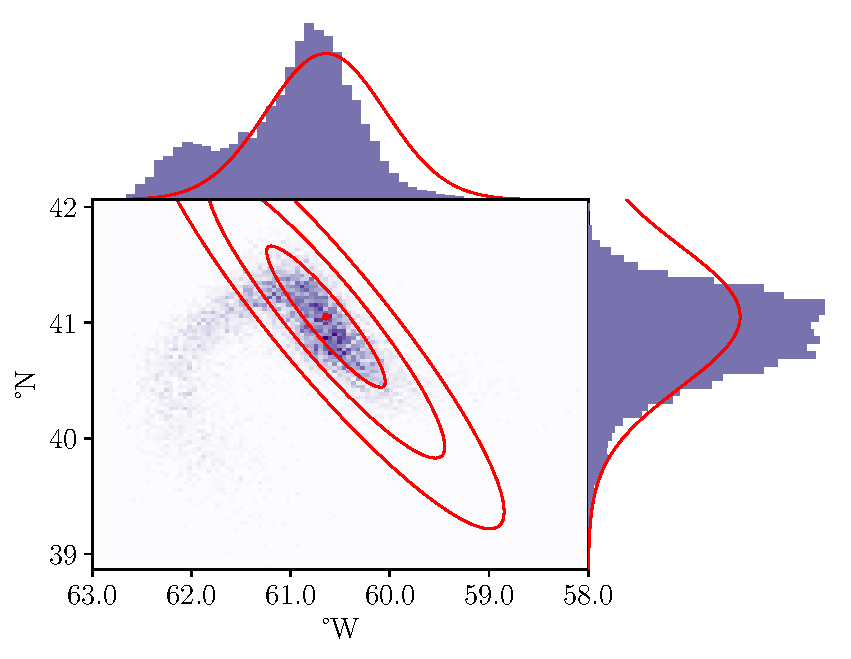
\includegraphics[width=\textwidth]{chp06_applications/figures/gulf_stream/traj_stoch_em_3.0}
			\caption{\(t = 3\) (midnight \DTMdisplaydate{2021}{01}{03}{-1})}
			\label{fig:natl_em_3}
		\end{subfigure}
		\begin{subfigure}{0.49\textwidth}
			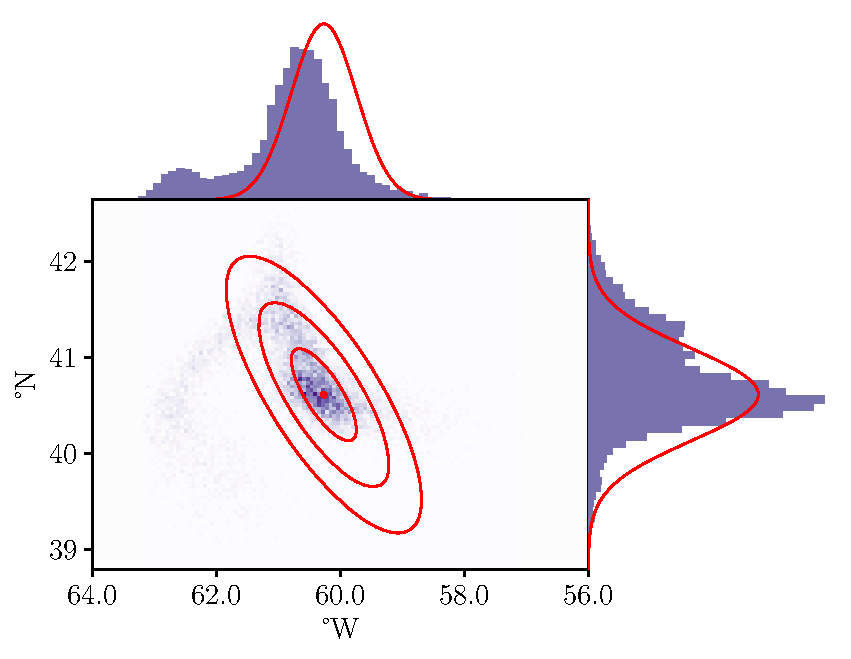
\includegraphics[width=\textwidth]{chp06_applications/figures/gulf_stream/traj_stoch_em_4.0}
			\caption{\(t = 4\) (midnight \DTMdisplaydate{2021}{01}{04}{-1})}
		\end{subfigure}
		\begin{subfigure}{0.49\textwidth}
			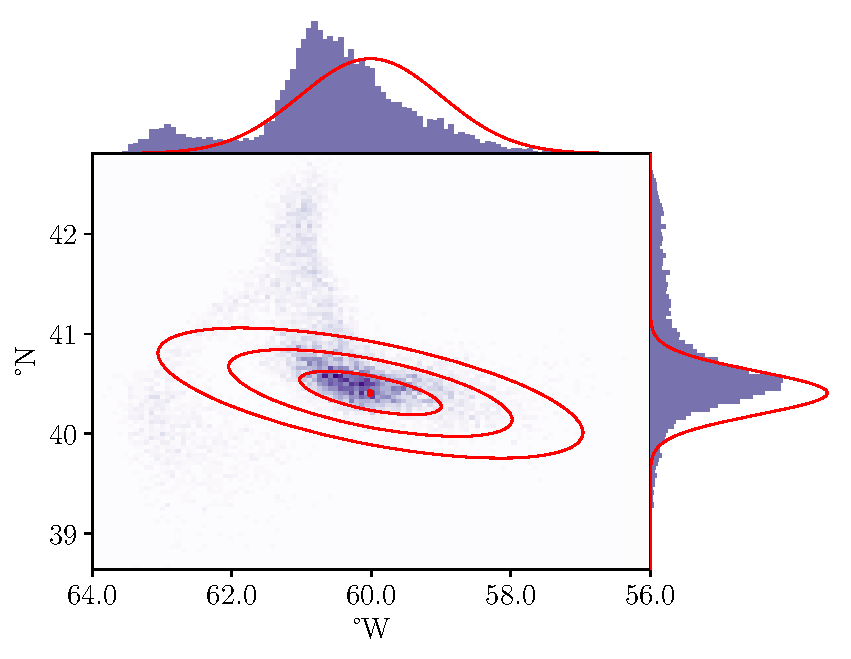
\includegraphics[width=\textwidth]{chp06_applications/figures/gulf_stream/traj_stoch_em_5.0}
			\caption{\(t = 5\) (midnight \DTMdisplaydate{2021}{01}{05}{-1})}
		\end{subfigure}
		\begin{subfigure}{0.49\textwidth}
			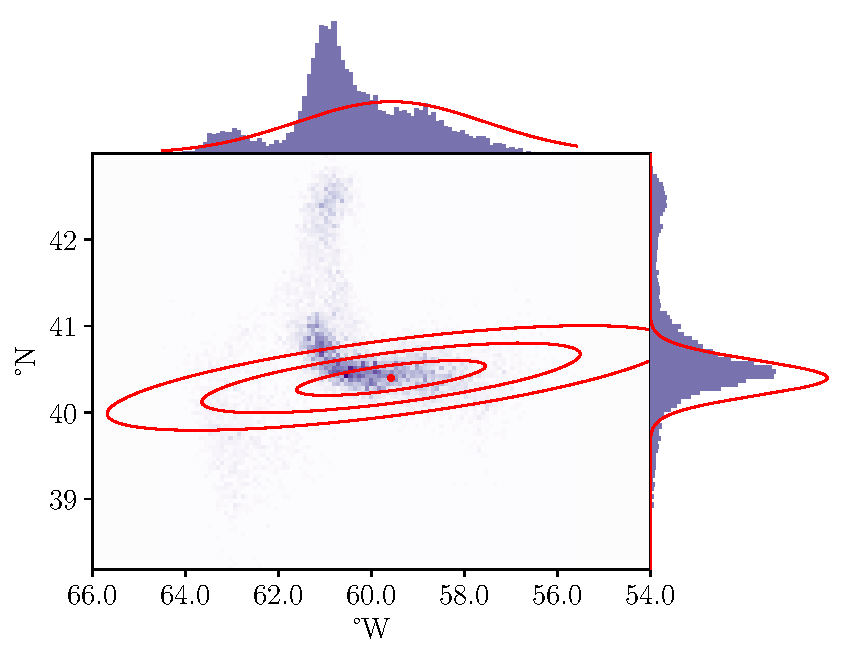
\includegraphics[width=\textwidth]{chp06_applications/figures/gulf_stream/traj_stoch_em_6.0}
			\caption{\(t = 6\) (midnight \DTMdisplaydate{2021}{01}{06}{-1})}
		\end{subfigure}
		\caption{The time-evolution of \(N = 10000\) Euler-Maruyama realisations of the solution to \cref{eqn:natl_sde}, with the Gaussian density arising from a linearisation of \cref{eqn:natl_sde} about the deterministic trajectory overlaid in red.
			The bivariate plot shows contours of the probability density function (or equivalently standard deviation bounds) of the Gaussian approximation, whereas each marginal plot on the longitudinal and latitudinal axis show the PDFs themselves of the Gaussian marginals.}
		\label{fig:natl_em}
	\end{center}
\end{figure}


The SDE \cref{eqn:natl_sde} is highly nonlinear and data-driven, so analytical solutions are not available.
However, we can compute a Gaussian approximation by linearising \cref{eqn:natl_sde} about the corresponding deterministic trajectory solving \cref{eqn:natl_ode} (with the same fixed initial condition), and employing the theory and computations of \Cref{ch:linear_theory}.
In \Cref{fig:natl_em}, we again plot histograms of the \(10000\) Euler-Maruyama realisations of the solution, and include marginal distributions in the longitudinal and latitudinal directions on each axis.
Overlaid in red is the Gaussian solution to the linearisation of \cref{eqn:natl_sde}.
The deterministic trajectory and covariance matrix are computed simultaneously using the Mazzoni method outlined in \Cref{sec:mazzoni}.
This computation requires the gradient of the velocity field, which we approximate with a centred finite difference.
In \Cref{fig:natl_em}, on each joint histogram, we have plotted contours of the bivariate Gaussian solution.
On each marginal histogram, we have plotted the probability density function of the marginal Gaussian corresponding to that component.
After a single day (\(t = 1\)), the numerical realisations match the Gaussian approximation, but the distribution of the realisations quickly becomes non-Gaussian due to both the nonlinearity of the flow and the multiplicative noise of the stochastic model.
While the large number of realisations that remain in the stream maintain a Gaussian-like shape with a single model, the scatter of trajectories leaving the stream results in a highly non-Gaussian distribution.
To account for this, the variance of the Gaussian approximation grows larger over time, particularly in the longitudinal direction.

\begin{figure}
	\begin{center}
		% \begin{subfigure}[t]{0.49\textwidth}
		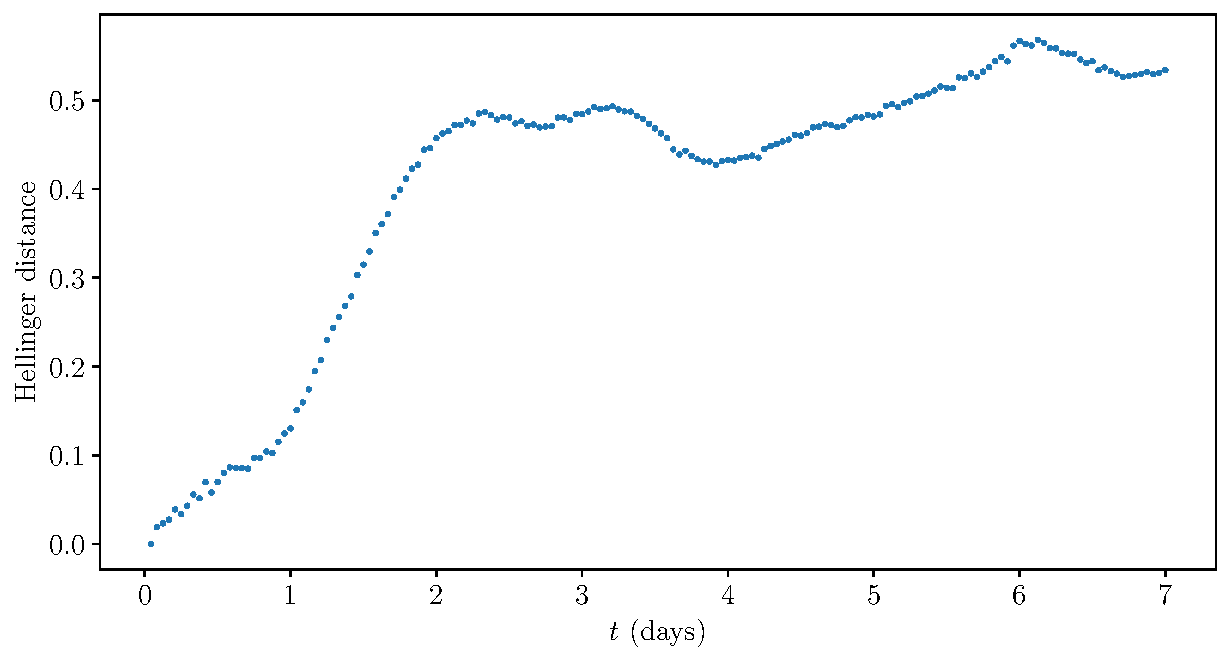
\includegraphics[width=\textwidth]{chp06_applications/figures/gulf_stream/traj_stoch_hell_dist_0.25}
		\caption{The estimated Hellinger distance between \(10000\) Euler-Maruyama samples of \cref{eqn:natl_sde} and the Gaussian process solution to the linearisation, \(t\) days after midnight \DTMdisplaydate{2021}{01}{01}{-1}.}
		\label{fig:natl_hell}
	\end{center}
\end{figure}

To quantitatively evaluate the quality of the Gaussian approximation over time, \Cref{fig:natl_hell} plots the estimated Hellinger distance between the Gaussian approximation and Euler-Maruyama samples solving \cref{eqn:natl_sde}.
We use 100 realisations of the Hellinger distance---that is, for each of those 100 calculations, we take \(10000\) new EM samples and \(10000\) samples of the Gaussian approximation and compute the empirical Hellinger distance with \cref{eqn:hell_emp}---and plot the average of these in \Cref{fig:natl_hell}.
The sample variance in this calculation is approximately \(\mathcal{O}\!\left(10^{-4}\right)\), so we do not include error bars in \Cref{fig:natl_hell} as they would be negligible.
% In \Cref{app:supp_hell_natl}, we provide additional figures showing the same computation, but for varying bin sizes, to verify that the Hellinger distance computation is reasonably robust to changes in this size.
% \td{Actually get this plots in there.}
As expected, the distance increases over time, as the numerical solution to \cref{eqn:natl_sde} quickly becomes non-Gaussian.
However, there are two times where the Gaussian approximation \emph{improves}: at \(t \approx 3.3\) and \(t \approx 6\).
This improvement may be because of contracting dynamics within the Gulf Stream, such as when the trajectories pass through the `bend' in the stream (evident around \(t = 3\) and \(t = 4\) in \Cref{fig:na_hist_t3}) which advect some realisations back towards each other.

The Gaussian solution to the linearisation can provide a reasonable representation of the drifter position distribution over short timeframes.
This linearisation solution still provides valuable insight into the stochastic system over longer periods of time, as we saw when computing the stochastic sensitivity field.
However, the highly non-linear dynamics of the system quickly drive the distribution away from the Gaussian distribution, and the aforementioned limitations of a Gaussian approximation, such as the inability to capture multiple modes and skew, become apparent.
The Gaussian approximation is still efficient to compute, however, so we will look to employ the Gaussian mixture model algorithm we described in \Cref{ch:gmm}.


\section{The mixture model}
We will explore a simple implementation of the mixture model algorithm described in \Cref{ch:gmm} to predict the distribution of stochastic solutions about the single trajectory in \Cref{sec:na_single}.
% Again, our aim is not to investigate the algorithm and model in detail, but to rather demonstrate the potential of this algorithm in efficiently approximating the stochastic solution.
As discussed in \Cref{ch:gmm}, we expect that the mixture model approach will work best in moderate noise models and over reasonably short timeframes.
We take the same fixed initial condition \(x_0 = \left(-60.5, 39\right)^{\T}\) but consider the position of the drifter at \(t = 3\), so at midnight \DTMdisplaydate{2021}{01}{04}{-1}.
The distribution of numerical samples at this time is given in \Cref{fig:natl_em_3}; the aim here is to use the mixture model algorithm to approximate this non-Gaussian distribution with a small number of Gaussian components, each constructed as solutions to the linearised SDE.
The two marginal distributions (in the longitudinal and latitudinal directions) in \Cref{fig:natl_em_3} demonstrate the qualitative departures from Gaussianity mentioned previously: in the longitudinal direction, the distribution of samples is bimodal, whereas in the latitudinal direction we see skew in the southern direction.
The distribution is 2-dimensional, however, so there are aspects of the joint density that are not reflected by the two marginal distributions, such as the curved structure of the density function.
This is a highly non-Gaussian distribution with distinct features that we would like to capture with a mixture model approximation.

\begin{figure}
	\centering
	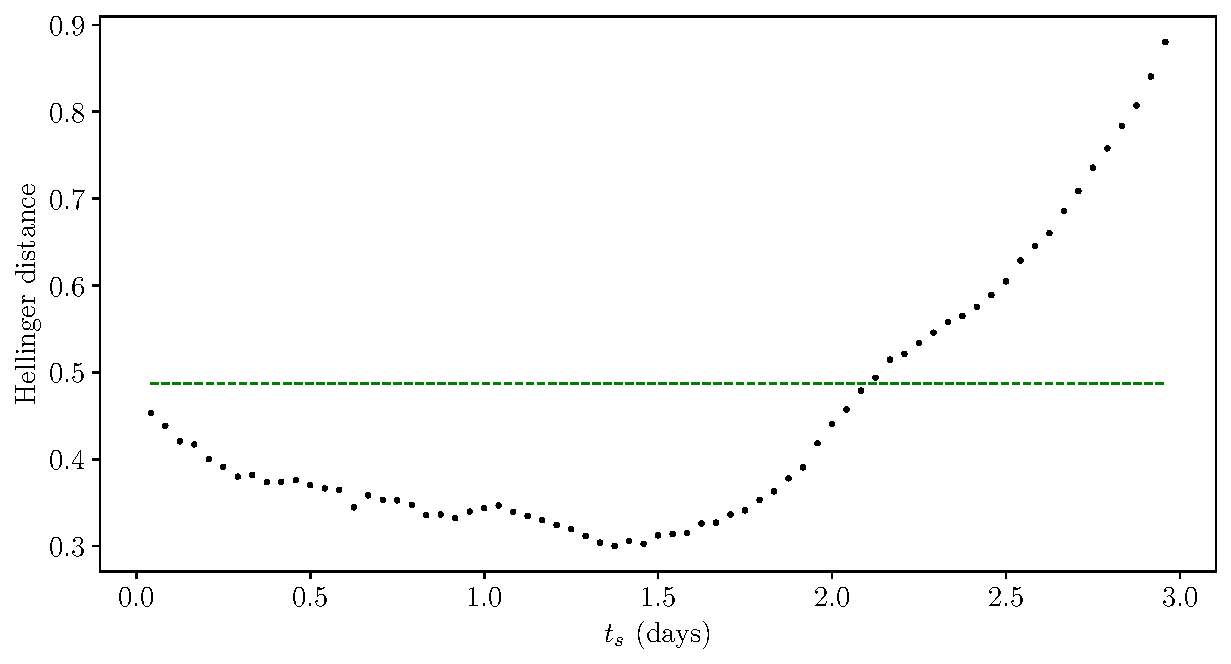
\includegraphics[width=\textwidth]{chp06_applications/figures/gulf_stream/hell_dist_split}
	\caption{The Hellinger distance between the mixture model implemented with a single split at time \(t_s\) and 10000 Euler-Maruyama samples of the solution to \Cref{eqn:natl_sde} at \(t = 3\).
		The green line indicates the Hellinger distance between the single Gaussian component and the samples.}
	\label{fig:na_1split_hell}
\end{figure}

First, we shall implement the GMM algorithm with a single manually specified split, for which we use the canonical sigma points \cref{eqn:uhlman_sigma} to split the covariance matrix at the specified time into 4 additional points.
With a single split, the mixture model comprises 5 equally weighted components: the original Gaussian component evolved from the initial condition, and the 4 additional components resulting from the splitting step.
For each splitting time, we can use the Hellinger distance between the resulting mixture model and the 10000 Euler-Maruyama realisations of the true solution to evaluate that choice of time.
This allows us to `tune' the choice of splitting time by finding that which results in the smallest distance.
This method, of course, relies upon us having already obtained the numerical samples over which we are trying to improve computational efficiency.
However, the purpose of this example is to demonstrate that such an optimal time can be found and to suggest that, once equipped with an appropriate online splitting criterion, the mixture model algorithm provides an efficient \emph{ad hoc} method for capturing key features of the distribution.
As a benchmark, the single Gaussian component (shown in \Cref{fig:natl_em_3} overlaid on the histograms of samples) gave a Hellinger distance of approximately 0.48761.
\Cref{fig:na_1split_hell} plots, against the split time \(t_s\), the Hellinger distance (averaged over 100 calculations) between each mixture model and a set of 10000 EM samples.
% The Hellinger distance between the single Gaussian approximation and the same EM samples is also indicated by the green line.
We can see that a split time earlier than \(t_s = 2\) results in a mixture model that improves over the single Gaussian approximation.
When the split occurs later, the quality of the resulting mixture model worsens.
The minimum Hellinger distance of approximately 0.30191 occurs with a split at \(t_s = 33/24\) days, or at 9am \DTMdisplaydate{2021}{01}{02}{-1}, which we take as our `best' fit.

\begin{figure}
	\centering
	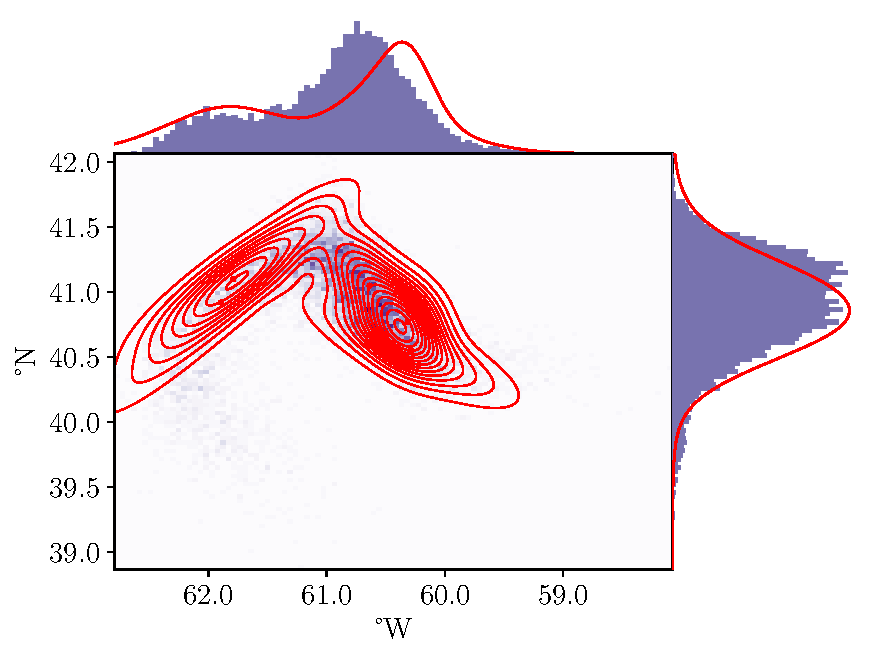
\includegraphics[width=\textwidth]{chp06_applications/figures/gulf_stream/gmm_split_best}
	\caption{The best-fitting mixture model with a single split at \(t_s = 33/24\) (9am \DTMdisplaydate{2021}{01}{02}{-1}).
		The joint histogram (centre) includes contours of the mixture probability density function.
		Each axis provides marginal histograms of the numerical samples, with the corresponding marginal PDFs of the mixture density in red.}
	\label{fig:na_1split_best}
\end{figure}


We compare the resulting mixture model against the numerical samples in \Cref{fig:na_1split_best}, in the same fashion as \Cref{fig:natl_em} where contours of the mixture probability density function are shown on the joint histogram and the marginal PDFs on each marginal histogram.
The mixture model captures several important qualitative features of the empirical distribution, including the bimodality in the longitudinal marginal and part of the `curved' shape of the joint distribution.
Comparing directly to the single Gaussian in \Cref{fig:natl_em_3}, the latitudinal marginal, with a smaller variance, more closely matches the spread of the samples.
However, the mixture fails to capture the full scatter of samples in the southern direction, even though this only corresponds to a small proportion of the samples.
Regardless, this result is promising, as with only a single split and four more components, we have improved over the single Gaussian approximation.

\begin{figure}
	\centering
	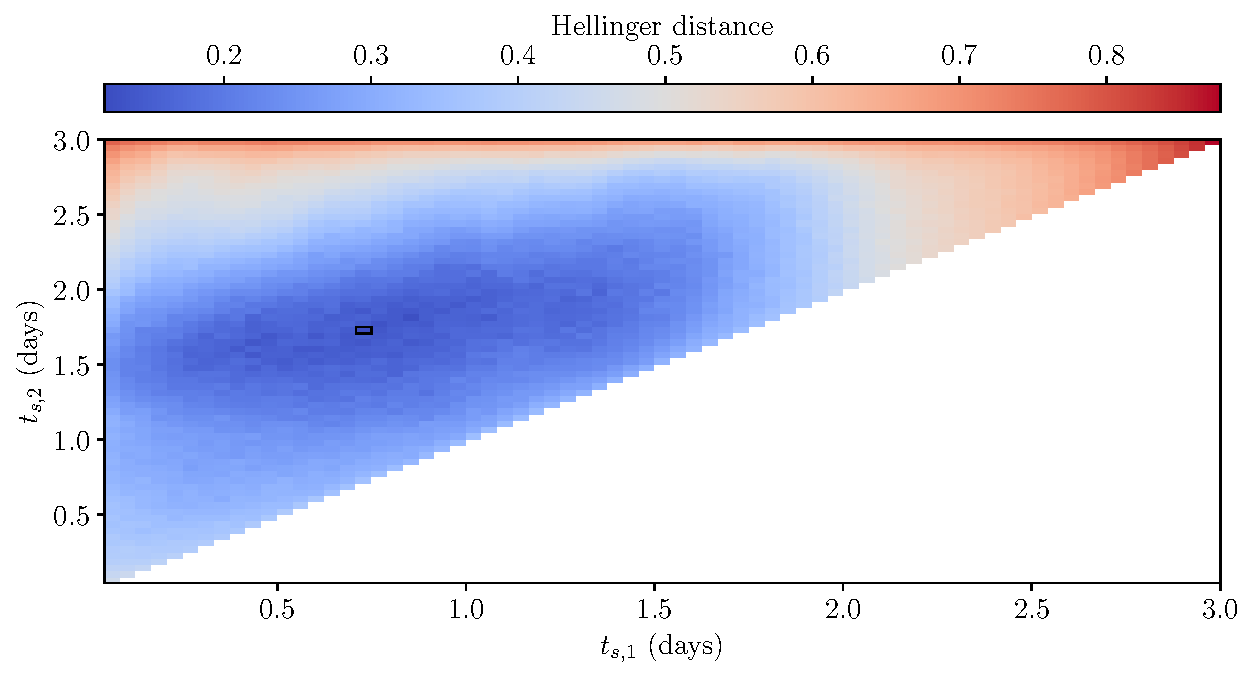
\includegraphics[width=\textwidth]{chp06_applications/figures/gulf_stream/hell_dist_2split}
	\caption{The Hellinger distance between the mixture model implemented with two splits---the first at \(t_{s,1}\) days, and the second at \(t_{s,2} > t_{s,1}\) days---and 10000 Euler-Maruyama samples of the solution to \cref{eqn:natl_sde} at \(t = 3\).
		When \(t_{s,1} = t_{s,2}\), the result for a single split at that time (from \Cref{fig:na_1split_hell}) is shown for comparison.
		The minimising value is indicated by the black box.}
	\label{fig:na_2split_hell}
\end{figure}


Five components may not be sufficient to fully capture the shape and spread of the empirical distribution, so we now consider adding an additional splitting step to each component.
After the first split at time \(t_{s,1}\), we will split each new trajectory at a later time \(t_{s,2}\).
For simplicity, each of the five trajectories is split at the \emph{same} time \(t_{s,2}\), but the algorithm allows for each trajectory to be split at different times as some regions may exhibit more Gaussianity than others.
Each component pair is split at time \(t_{s,2}\) into four additional points, again using the canonical sigma points \cref{eqn:uhlman_sigma} to preserve the mean and covariance.
We consider a range of times for \(t_{s,1}\) and \(t_{s,2}\), construct the mixture model using each pair of times, and compute the empirical Hellinger distance (again averaged over 100 calculations) between the mixture density and the EM samples to find the best configuration.
The resulting Hellinger distances are shown in \Cref{fig:na_2split_hell}.
The optimal configuration with two splits has the first at \(t_{s,1} = 3/4\) (at 6pm \DTMdisplaydate{2021}{01}{01}{-1}) and the second at \(t_{s,2} = 43/24\) (at 7pm \DTMdisplaydate{2021}{01}{02}{-1}), and results in a Hellinger distance of approximately 0.14684.
This distance is a substantial improvement over both the single Gaussian component and the mixture model with a single split.

\begin{figure}
	\centering
	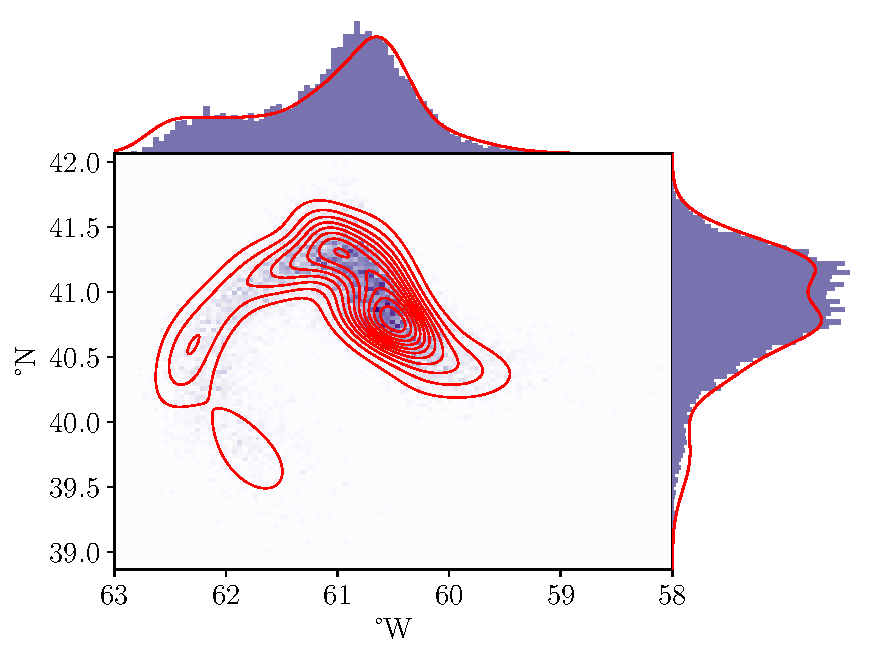
\includegraphics[width=\textwidth]{chp06_applications/figures/gulf_stream/gmm_2split_best}
	\caption{The best-fitting mixture model (in red) with two splits on each component, over histograms of 10000 Euler-Maruyama samples.
		The central joint histogram shows contours of the mixture probability density function.
		On the longitudinal and latitudinal marginals on each axis, the probability density functions of the corresponding marginals of the mixture model are shown.}
	\label{fig:na_2split_best}
\end{figure}

In \Cref{fig:na_2split_best}, we compare this mixture density against the stochastic samples.
The mixture model captures the shape of the empirical distribution, including the scatter of points leaving the stream in the westward direction.
The bimodality in the longitudinal marginal and the skew in the latitudinal are captured by the mixture model.
The 25-component mixture model provides a close representation of the empirical distribution, both heuristically (by capturing qualitative departures from Gaussianity) and supported by the small Hellinger distance of 0.14684.
Whereas we propagated 10000 Euler-Maruyama samples to construct the empirical distribution, the mixture model comprises only 25 mean-covariance pairs, the computation of which can be thought of as requiring the propagation of only 125 values (the two components of each mean and the three components of each symmetric covariance matrix).
A mixture model with fewer components (by having fewer splits in total) may also provide the same quality of approximation, which would be even more computationally efficient.
Estimating the true solution distribution is a difficult problem, as the deterministic dynamics are complicated and highly non-linear, and the non-uniformity of error in the observations used to construct it means that the noise is multiplicative.
With a simple implementation of the mixture model, we can capture key features and provide a close approximation of the distribution of the solution at \(t = 3\).
Evaluating the mixture model and finding the best splitting times required a set of numerical realisations of the SDE solution when our overall aim is to avoid this computational cost.
However, we continue to emphasise that this example is demonstrative and the mixture model has only been proposed as an outline of an algorithm.
Nonetheless, the results of this section are encouraging and motivate further development and investigation of the algorithm.
% There are clear splitting times in \Cref{fig:na_1split_hell,fig:na_2split_hell} for which the mixture model results in an optimal (with respect to the Hellinger distance) fit.\td{Need to articulate this better.}
Once equipped with an appropriate splitting criterion, the mixture model algorithm could become a highly effective method for circumventing bulk simulation in stochastic systems.
Even without this splitting criterion, the mixture model provides an explicit form for the probability density function, which may lend itself to further applications.
% We discuss this in \Cref{sec:gmm_extensions}.



% \section{Empirical model of sea-surface winds}
% \td{Possibly something funky to try - use the observed data to construct the FLOW MAP, and then compute based purely on that!! The paper by \cite{Sura_2003_StochasticAnalysisSouthern} basically interpolates the data then uses finite differences and statistical averaging to find the ODE. But we can avoid that step entirely by just treating the data!}

% Empirical, or data-driven, stochastic models are used heavily in climate science, where components of the model are derived by fitting to time series of observed data.
% In this section, we follow the method of \citet{EggerJonsson_2002_DynamicModelsIcelandic} and \citet{Sura_2003_StochasticAnalysisSouthern} to construct from observed data a stochastic differential equation model for the time evolution of sea surface wind velocities.

% Consider an \(n\)-dimensional state variable \(x_t\) governed by the It\^o SDE
% \begin{equation}\label{eqn:sde_emp}
% 	\dif x_t = A(x_t) + B(x_t)\dif W_t,
% \end{equation}
% where \(W_t\) is an \(n\)-dimensional Wiener process and the coefficients \(A \colon \R^n \to \R^n\) and \(B \colon \R^n \to \R^{n\times n}\) are permitted to vary with state but not time.
% To determine the drift and diffusion directly from observed data, we consider the statistical definitions of the coefficients:
% \begin{subequations}\label{eqn:sde_coef_stat}
% 	\begin{align}
% 		A(x)          & = \lim_{\delta t \to 0}\frac{1}{\delta t}\avg{x_{t + \delta t} - x} \label{eqn:sde_coef_stat_drift}                                                \\
% 		B(x)B(x)^{\T} & = \lim_{\delta t \to 0}\frac{1}{\delta t}\avg{\left(x_{t + \delta} - x\right)\left(x_{t + \delta} - x\right)^{\T}}, \label{eqn:sde_coef_stat_diff}
% 	\end{align}
% \end{subequations}
% where the expected values are taken over all trajectories solving \cref{eqn:sde_emp} with \(x_{t} = x\).
% The expressions in \cref{eqn:sde_coef_stat} arise by considering the Fokker-Planck equation corresponding to \eqref{eqn:sde_emp} \citehere.

% Now suppose that we have a collection of \(K\) time series, each corresponding to a solution trajectory of \cref{eqn:sde_emp} and evaluated at (possibly non-uniform) times \(t_0, t_1, \dotsc, t_n\).
% Let the \(k\)th time series be denoted by
% \[
% 	\set{X_{0}^{(k)}, X_{1}^{(k)}, \dotsc, X_{n}^{(k)}}.
% \]
% The definitions in \cref{eqn:sde_coef_stat} are only correct in the limit as \(\delta t\) approaches zero, which we cannot obtain from our discrete-time data, and involves expectations of the theoretical solution to \eqref{eqn:sde_emp}.
% However, we can approximate the expressions using a finite difference for the limit and binned sample estimates for the expectations.




% \section{Epidemiology}



% Stochastic differential equations emerge from these discrete models in the limit of an infinite population size.
% Analogous to the behaviour of nonlinear stochastic differential equations in small noise limits (as established by \citet{FreidlinWentzell_1998_RandomPerturbationsDynamical} and our work in \Cref{ch:linear_theory}), the density process converges to the solution to a system of ordinary differential equations (known as the \emph{fluid limit} in some literature).
% Moreover, the stochastic variation of the process about this deterministic limit converges to the solution to a linear stochastic differential equation (known as the \emph{diffusion limit}).
% We summarise these results in \Cref{sec:epi_limits}.




% \subsection{A very brief overview of population processes}
% A common model for population process are continuous-time Markov chains (CTMCs)
% Here, we provide only a brief overview of population processes; for a more detailed intorduction, see \citehere.

% The population process is described by the transition function \(q\colon \mathcal{S}\times\mathcal{S} \to [0,\infty)\), where \(q(x,y)\) describes the rate at which

% A single sample \(X\) from the population process at time \(T\) can be simulated with the following procedure \citep{Gillespie_1977_ExactStochasticSimulation}:
% \begin{enumerate}
% 	\item Initialise \(X = X_0\), the initial state of the process.
% 	      If the initial state is uncertain, sample \(X\) from the initial state distribution.

% 	\item Sample the time \(\tau\) to the next event as
% 	      \[
% 		      \tau \isExp{\sum_{\substack{l \in \R^n \\ l \neq 0,\, y + l \in \mathcal{S}}}{q\!\left(X, X + l\right)}},
% 	      \]
% 	      and set \(t = t + \tau\).

% 	\item If \(t > T\), terminate.
% 	      Otherwise, sample the next state from the set of possible transitions \(\setc{l \in \R^n}{l \neq 0,\, y + l \in \mathcal{S}}\), where the probability of transitioning from \(X\) to \(X + l\) is given by
% 	      \[
% 		      \frac{q\!\left(X, X + l\right)}{\sum_{\substack{k \in \R^n \\ k \neq 0,\, y + k \in \mathcal{S}}}{q\!\left(X, X + k\right)}}.
% 	      \]
% 	      Set \(X\) to this state.

% 	\item Repeat Steps 2 and 3 until the sample path is terminated.

% \end{enumerate}
% The result is a single sample \(X\) of the population process at time \(T\).
% The sum is taken across all the possible transitions from the current state.
% Note that typically most of these rates are zero, so the sum does not need to be taken over the entire state space.

% \subsection{Large population diffusion limits}\label{sec:epi_limits}
% In the limit of large population sizes, a deterministic ordinary differential equation and linear stochastic differential equation arise from certain population processes, despite these processes being discrete.
% A population process is \emph{density dependent} (in the sense of \citet{Kurtz_1970_SolutionsOrdinaryDifferential}) if there is a parameter \(N\) such that
% \begin{equation}
% 	q\!\left(n, n+l\right) = Nf\!\left(\frac{n}{N}, l\right),
% 	\label{eqn:ctmc_dens_dep}
% \end{equation}
% where \(f\) is a suitable function and \(n, n+l \in \mathcal{S}\).
% Typically, \(N\) is related to the size of the system and \(n / N\) is a population density.
% The condition in \cref{eqn:ctmc_dens_dep} states that the transition rates of the process \(X_t\) depends on \(X_t\) itself only through the density \(X_t / N\).

% Let \(Y_t^{(N)}\) describe the \(n\)-dimensional density process, i.e. with \(i\)th element \(X_t^{(i)} / N\).
% Theorem 3.1 of \citet{Kurtz_1970_SolutionsOrdinaryDifferential} establishes that in the large population limit \(N \to \infty\), the density process \(Y_t^{(N)}\) converges in probability to a deterministic trajectory \(Y_t^{(\infty)}\) solving the ODE
% \begin{equation}
% 	\dod{Y_t^{(\infty)}}{t} = Q\!\left(Y_t^{(\infty)}\right), \quad Y_0^{(\infty)} = X_0 / N,
% 	\label{eqn:ctmc_dens_dep_ode}
% \end{equation}
% where
% \[
% 	Q\!\left(y\right) = \sum_{\substack{l \in \R^n \\ l \neq 0,\, y + l \in \mathcal{S}}}{l f\!\left(y, l\right)}.
% \]
% For large \(N\), the density process has small variation and is ``close'' to the deterministic solution to \cref{eqn:ctmc_dens_dep_ode}.
% This result is analogous to that for small noise SDEs; the solution to a stochastic differential equation formally converges to that of a deterministic system (involving only the drift term) in the limit of small noise, which is a result established by large deviations principles \citep[e.g]{FreidlinWentzell_1998_RandomPerturbationsDynamical}.

% \citet{Kurtz_1971_LimitTheoremsSequences} then established a stronger result, showing that the variation of the density process about this deterministic limit is captured by an It\^o diffusion.
% Define the scaled process
% \[
% 	Z_t^{(N)} = \sqrt{N}\left(Y_t^{(N)} - Y_{t}^{(\infty)}\right),
% \]
% then Theorem 3.5 of \citet{Kurtz_1971_LimitTheoremsSequences} proves that \(Z_t^{(N)}\) converges in distribution (weakly) to an It\^o diffusion \(Z_t^{(\infty)}\) solving
% \begin{equation}
% 	\dif Z_t^{(\infty)} = \nabla Q\!\left(Y_t^{(\infty)}\right) Z_t^{(\infty)}\dif t + G\!\left(Y_t^{(\infty)}\right)\dif W_t, \quad Z_0^{(\infty)} = 0,
% 	\label{eqn:ctmc_dens_dep_sde}
% \end{equation}
% where \(W_t\) is an \(n\)-dimensional Wiener process and the \(n \times n\) diffusion matrix \(G\) is such that
% \begin{equation}
% 	\left[G\!\left(y\right)G\!\left(y\right)^{\T}\right]_{ij} = \sum_{\substack{l \in \R^n \\ l \neq 0,\, y + l \in \mathcal{S}}}{l_i l_j f\!\left(y,l\right)}
% 	\label{eqn:ctmc_dens_dep_sde_diff_cond}
% \end{equation}
% Any choice of diffusion matrix \(G\) such that \cref{eqn:ctmc_dens_dep_sde_diff_cond} is satisfied will result in a statistically identical diffusion process \(Z_0^{(\infty)}\).

% The limiting SDE \cref{eqn:ctmc_dens_dep_sde} is equivalent to the unscaled SDE
% \begin{equation}
% 	\dif L_t^{(N)} = \left[Q\!\left(Y_t^{(\infty)}\right) + \frac{1}{\sqrt{N}} \nabla Q\!\left(Y_t^{(\infty)}\right)\left(L_t^{(N)} - Y_t^{(\infty)}\right)\right]\dif t + \frac{1}{\sqrt{N}}G\!\left(Y_t^{(\infty)}\right)\dif W_t,
% 	\label{eqn:ctmc_sde_lin_lim}
% \end{equation}
% which is a linearisation of the nonlinear SDE
% \begin{equation}
% 	\dif \hat{Y}^{(N)}_t = Q\!\left(\hat{Y}^{(N)}_t\right)\dif t + \frac{1}{\sqrt{N}}G\!\left(\hat{Y}_t^{(N)}\right)\dif W_t
% 	\label{eqn:ctmc_sde_lim_nonlin}
% \end{equation}
% about the deterministic limit \(Y_t^{(\infty)}\).
% There is intuition behind the choices of drift and diffusion in \cref{eqn:ctmc_sde_lim_nonlin}.
% For sufficiently large \(N\), the drift term \(Q\) captures the average (macroscopic) behaviour of the density process.
% The diffusion term captures the microscopic behaviour resulting from individual transition events, and the uncertainty in this is parameterised with the Wiener process \(W_t\).




% \td{Explain how this is analogous to the proceeding work}
% However, a key difference is that in the SDE linearisation procedure, we start from a continuous state-space process and arrive at a continuous state-space process in the limit.
% Whereas, in the CTMC diffusion limit, the converging process is on a \emph{discrete} state-space and the limit is on a continuous one.




% Thus, we expect that the mixture model algorithm we have described may find a place in moderate-population compartmental models, where the population is large enough to be ``reasonably'' approximated by the continuum and SDE equations, but small enough to exhibit non-Gaussian behaviour.
% Regardless, our error bound derived in \Cref{ch:linear_theory} still has a place in this literature.



% \subsection{Example 1: the SIR model}
% Assume a fixed population of \(N\) individuals, each classified into one of three compartments: susceptible (\(S\)) and infected (\(I\)), and recovered/removed (\(R\)).
% At any time, the number of removed individuals can be computed as \(R = N - S - I\), so we only need to specify a two-dimensional model for the number of susceptible and infected individuals.
% Such a process can model the spread of a disease in a homogeneously mixing population in which susceptible individuals become infected upon contact with infected individuals, and once infected individuals recover they are no longer infectious or susceptible to reinfection.
% The state space is then
% \[
% 	\mathcal{S} = \setc{\left(s,i\right)}{s,i \in \set{0,1,\dotsc,N}, \, s + i \leq N},
% \]
% where the number of recovered individuals at any time is \(N - S - I\).
% The events and the corresponding transition probabilities are described in \Cref{fig:sir_transition}.

% \usetikzlibrary{automata,positioning,arrows}
% \tikzset{->, node distance = 2cm}
% \begin{figure}
% 	\begin{center}
% 		\begin{tabular}{|c|c|c|c|}
% 			\hline
% 			Transition & \multicolumn{2}{c|}{Event} & Rate \(\lambda_i\)                                                    \\ \hline
% 			1          & Infection                  & \(\left(S, I\right) \to \left(S-1, I + 1\right)\) & \(\beta S I / N\) \\ \hline
% 			2          & Recovery                   & \(\left(S,I\right) \to \left(S, I - 1\right)\)    & \(\gamma I\)      \\ \hline
% 		\end{tabular} \\
% 		\begin{tikzpicture}
% 			\node[state] (S) {\(S\)};
% 			\node[state, right of = S] (I) {\(I\)};
% 			\node[state, right of = I] (R) {\(R\)};
% 			\draw (S) edge[above] node{(1)} (I)
% 			(I) edge[above] node{(2)} (R);
% 		\end{tikzpicture}
% 		\caption{Transition probabilities of the SIR compartmental model.}
% 		\label{fig:sir_transition}
% 	\end{center}
% \end{figure}
% The population process is density dependent, with
% \[
% 	f\left((s,i), l\right) = \begin{cases}
% 		\beta s i, & \text{if } l = \left(-1, 1\right), \\
% 		\gamma i,  & \text{if } l = \left(0,-1\right)   \\
% 		0,         & \text{otherwise}.
% 	\end{cases}
% \]
% Let \(X_t^{(N)} = \left(S_t / N, I_t / N\right)\) denote the proportion of susceptible and infected individuals and at time \(t\).
% The corresponding deterministic differential equation approximation is
% \[
% 	\dod{X_t^{(\infty)}}{t} = \begin{bmatrix}
% 		-\beta X_t^{(\infty,1)} X_t^{(\infty, 2)} \\
% 		\beta X_t^{(\infty,1)} X_t^{(\infty, 2)} -\gamma X_t^{(\infty, 2)}
% 	\end{bmatrix},
% \]
% where \(X_t^{(\infty)} \equiv \left(X_t^{(\infty, 1)}, X_t^{(\infty, 2)}\right)^{\T}\).
% Consider the scaling
% \[
% 	Z_t^{(N)} = \sqrt{N}\left(X_t^{(N)} - X_t^{(\infty)}\right),
% \]
% then \citet{Kurtz_1971_LimitTheoremsSequences} establish that in the limit \(N \to \infty\), the scaled process \(Z_t^{(N)}\) will converge in distribution to the It\^o diffusion \(Z_t^{(\infty)}\) solving
% \begin{equation}
% 	\dif Z_t^{(\infty)} = \begin{bmatrix}
% 		-\beta X_t^{(\infty, 2)} & -\beta X_t^{(\infty, 1)}         \\
% 		\beta X_t^{(\infty, 2)}  & \beta X_t^{(\infty, 1)} - \gamma
% 	\end{bmatrix} Z_t^{(\infty)}\dif t + g\!\left(X_t^{(\infty)}\right)\dif W_t
% 	\label{eqn:sir_diff_limit}
% \end{equation}
% where the diffusion matrix \(G\) satisfies
% \[
% 	g\!\left(X_t^{(\infty)}\right)g\!\left(X_t^{(\infty)}\right)^{\T} = \begin{bmatrix}
% 		\beta X_t^{(\infty, 1)} X_t^{(\infty, 2)}  & -\beta X_t^{(\infty, 1)} X_t^{(\infty, 2)}                              \\
% 		-\beta X_t^{(\infty, 1)} X_t^{(\infty, 2)} & \beta X_t^{(\infty, 1)} X_t^{(\infty, 2)} + \gamma X_{t}^{(\infty, 2)}.
% 	\end{bmatrix}
% \]
% Any choice of \(g\) satisfying this property will result in a statistically identical diffusion process, so we take
% \[
% 	g\!\left(X_t^{(\infty)}\right) = \begin{bmatrix}
% 		\sqrt{\beta X_t^{(\infty, 1)} X_t^{(\infty, 2)}}  & 0                               \\
% 		-\sqrt{\beta X_t^{(\infty, 1)} X_t^{(\infty, 2)}} & \sqrt{\gamma X_t^{(\infty, 2)}}
% 	\end{bmatrix}.
% \]
% The stochastic differential equation \cref{eqn:sir_diff_limit} is a linear in the same form as the linearisation \cref{eqn:linear_sde} considered in \Cref{ch:linear_theory}, and so is solved by the Gaussian process
% \[
% 	Z_t^{(\infty)} \isGauss{0,\, \Sigma_0^t\!\left(X_0^{(\infty)}\right)},
% \]
% where \(\Sigma_0^t\!\left(X_0^{(\infty)}\right)\) is the symmetric positive-definite solution to the matrix differential equation
% \[
% 	\dod{\Sigma_0^t\!\left(X_0^{(\infty)}\right)}{t} = \begin{multlined}[t]
% 		\begin{bmatrix}
% 			-\beta X_t^{(\infty, 2)} & -\beta X_t^{(\infty, 1)}         \\
% 			\beta X_t^{(\infty, 2)}  & \beta X_t^{(\infty, 1)} - \gamma
% 		\end{bmatrix}\Sigma_0^t\!\left(X_0^{(\infty)}\right) \\
% 		+ \Sigma_0^t\!\left(X_0^{(\infty)}\right)\begin{bmatrix}
% 			-\beta X_t^{(\infty, 2)} & \beta X_t^{(\infty, 1)}          \\
% 			-\beta X_t^{(\infty, 2)} & \beta X_t^{(\infty, 1)} - \gamma
% 		\end{bmatrix} \\
% 		+ \begin{bmatrix}
% 			\beta X_t^{(\infty, 1)} X_t^{(\infty, 2)}  & -\beta X_t^{(\infty, 1)} X_t^{(\infty, 2)}                              \\
% 			-\beta X_t^{(\infty, 1)} X_t^{(\infty, 2)} & \beta X_t^{(\infty, 1)} X_t^{(\infty, 2)} + \gamma X_{t}^{(\infty, 2)}.
% 		\end{bmatrix}.
% 	\end{multlined}
% \]

% For the purposes of this demonstrative example, take the rate of infection to be \(\beta = 1.2\) and the rate of recovery to be \(\gamma = 0.8\).
% These values correspond to a reproductive number of \(R_0 = 1.5\), meaning that in the early stage of the population process, a single infected individual results in an average of 1.5 new infections.

% We first show that stochastic simulations of the density process for the SIR model converge to the Gaussian process solving \cref{eqn:sir_diff_limit}, in a similar manner to how we validated our convergence results for stochastic differential equations in \Cref{ch:linear_numerics}.
% For several different population sizes, we generate \(100000\) Monte-Carlo realisations of the CTMC SIR process at time \(t = 5\) and plot histograms of the corresponding density processes in \Cref{fig:sir_gauss_rels}.
% Each population process is initialised with 10\% of the \(M\) individuals infected and the remaining 90\% susceptible.
% For large populations (\(M = 1000\) and \(M = 10000\)), the diffusion limit appears to provide a reasonable approximation for the density process, as expected from the theory of \citet{Kurtz_1970_SolutionsOrdinaryDifferential,Kurtz_1971_LimitTheoremsSequences}.
% We therefore also expect that our developments using the Gaussian process solution to a linearised SDE can be applied in these situations.
% \td{Fix alignments in histograms.}

% \begin{figure}
% 	\begin{center}
% 		\begin{subfigure}{0.49\textwidth}
% 			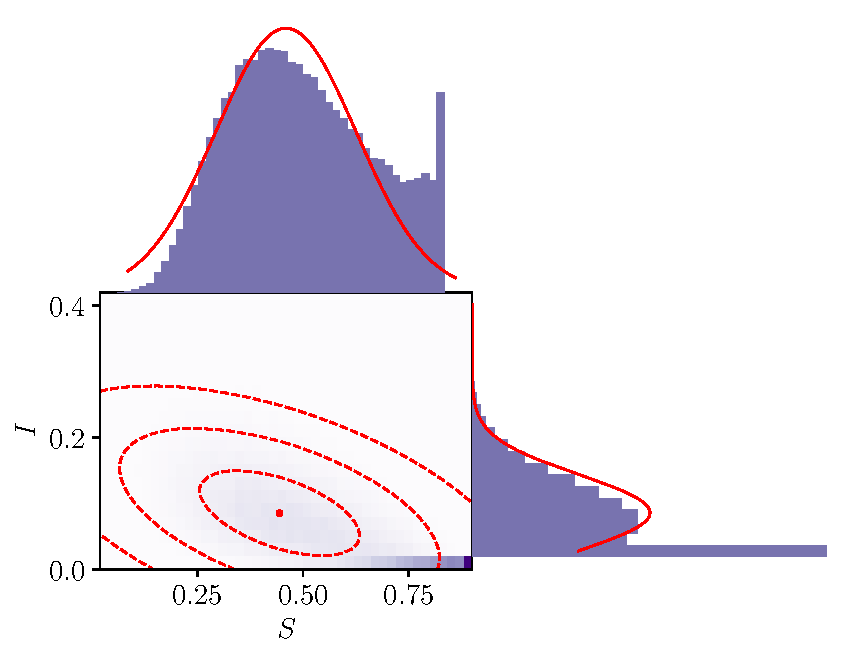
\includegraphics[width=\textwidth]{chp06_applications/figures/sir/sir_pairwise_50}
% 			\caption{\(M = 50\)}
% 			\label{fig:sir_gauss_rels_1}
% 		\end{subfigure}
% 		\begin{subfigure}{0.49\textwidth}
% 			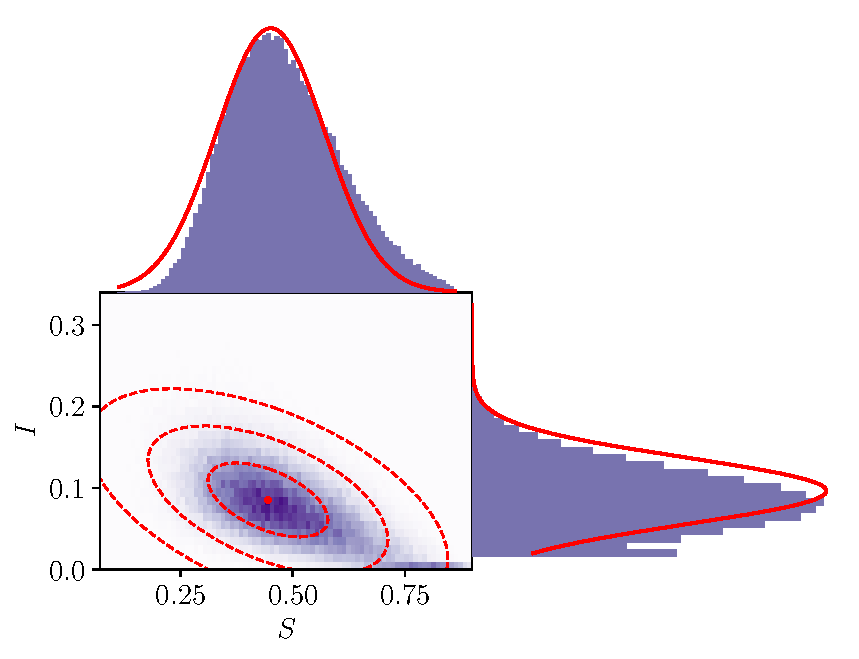
\includegraphics[width=\textwidth]{chp06_applications/figures/sir/sir_pairwise_100}
% 			\caption{\(M = 100\)}
% 			\label{fig:sir_gauss_rels_2}
% 		\end{subfigure}
% 		\begin{subfigure}{0.49\textwidth}
% 			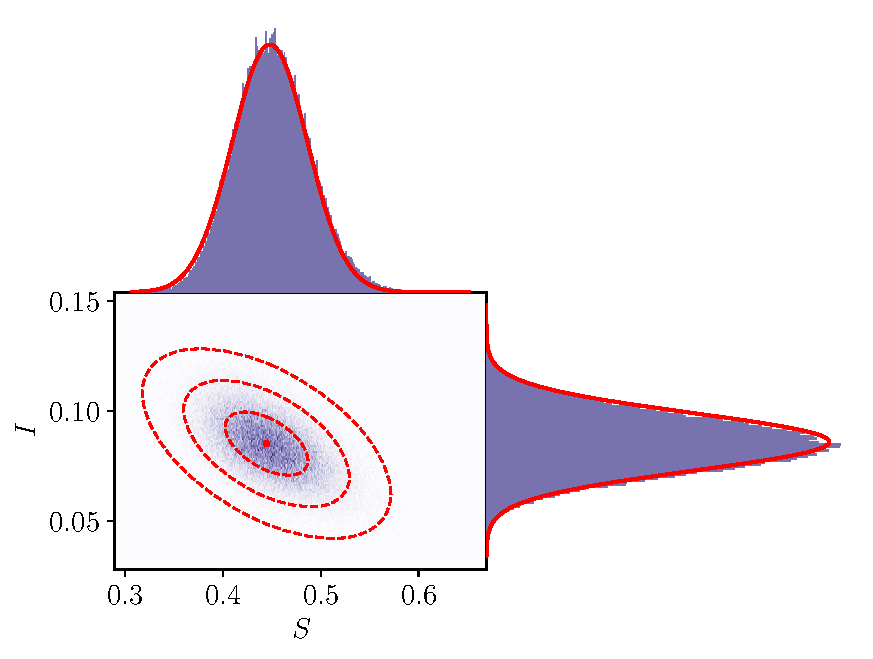
\includegraphics[width=\textwidth]{chp06_applications/figures/sir/sir_pairwise_1000}
% 			\caption{\(M = 1000\)}
% 			\label{fig:sir_gauss_rels_3}
% 		\end{subfigure}\begin{subfigure}{0.49\textwidth}
% 			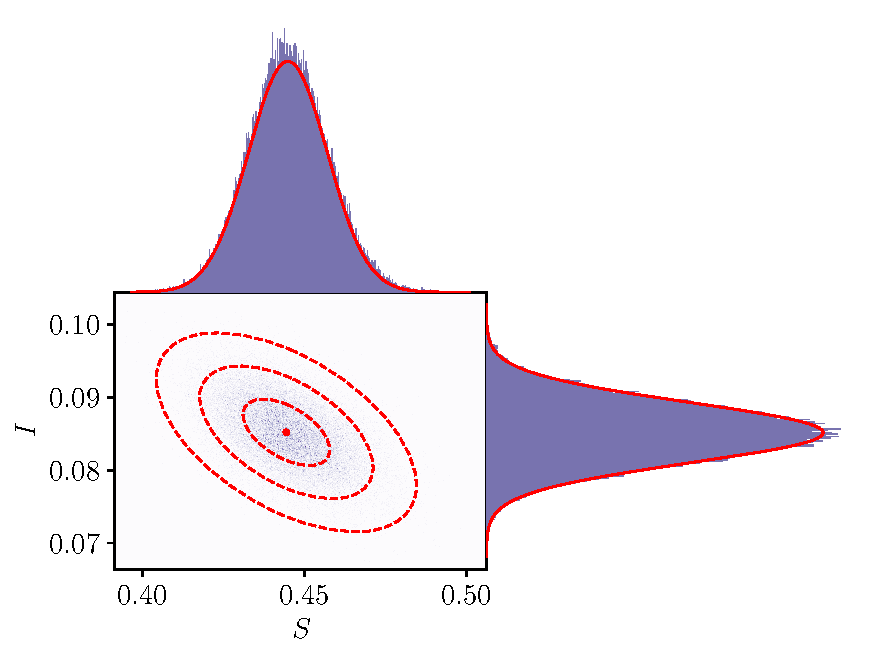
\includegraphics[width=\textwidth]{chp06_applications/figures/sir/sir_pairwise_10000}
% 			\caption{\(M = 10000\)}
% 			\label{fig:sir_gauss_rels_4}
% 		\end{subfigure}
% 		\caption{Histograms of Monte-Carlo simulations of the density process for the SIR model (with marginal plots on each axis), and the probability density function of the corresponding solution to the diffusion limit \cref{eqn:sir_diff_limit} plotted in red.
% 			Each sample path is initialised with 10\% of the population infected (i.e. \(x_0 = \left(0.1, 0.9\right)^{\T}\)).}
% 		\label{fig:sir_gauss_rels}
% 	\end{center}
% \end{figure}

% However, \Cref{fig:sir_gauss_rels} also highlights the limitations of using Gaussian approximations for certain types of stochastic processes.
% An \(n\)-dimensional Gaussian random variable has support on the entirety of \(\R^n\); that is, for any non-empty subset of \(\R^n\), there is a non-zero probability of the variable taking a value in that set.
% However, in many situations we can enforce (often from physical considerations) boundary conditions on the state variable.
% In the SIR model, the \(I = 0\) and \(S = 0\) boundaries are \emph{absorbing}, in the sense that once the stochastic process reaches those states, it remains there indefinitely with probability \(1\).
% We also saw another example of boundaries in the Gulf Stream example in \Cref{sec:appl_ocean}; the dataset only contained velocity
% Boundary issues were avoided by ensuring that the evolution of the deterministic trajectory was sufficiently far from the boundaries and the scale of uncertainty small enough so that the probability of a stochastic trajectory nearing the boundary is negligible.



% For large populations, the Gaussian diffusion limit is a well-used approximation that has been employed across many different modelling scenarios \citep[e.g.]{PollettEtAl_2010_ModellingPopulationProcesses}.
% Rather, we are interested in the moderate-sized population case where the population is large enough to limit the practicality of Monte-Carlo simulation, but is small enough that the density process distributions demonstrate departures from Gaussianity.
% Our aim is to employ the GMM algorithm to provide computationally efficient approximations in these scenarios, which we explore on a 5-dimensional example informed by real data in the next section (\Cref{sec:epi_5d}).

% Next, we will compute the stochastic sensitivity field on the set of (physically relevant) initial conditions to the SIR model.



% \begin{figure}
% 	\begin{center}
% 		% \begin{subfigure}{0.49\textwidth}
% 		% 	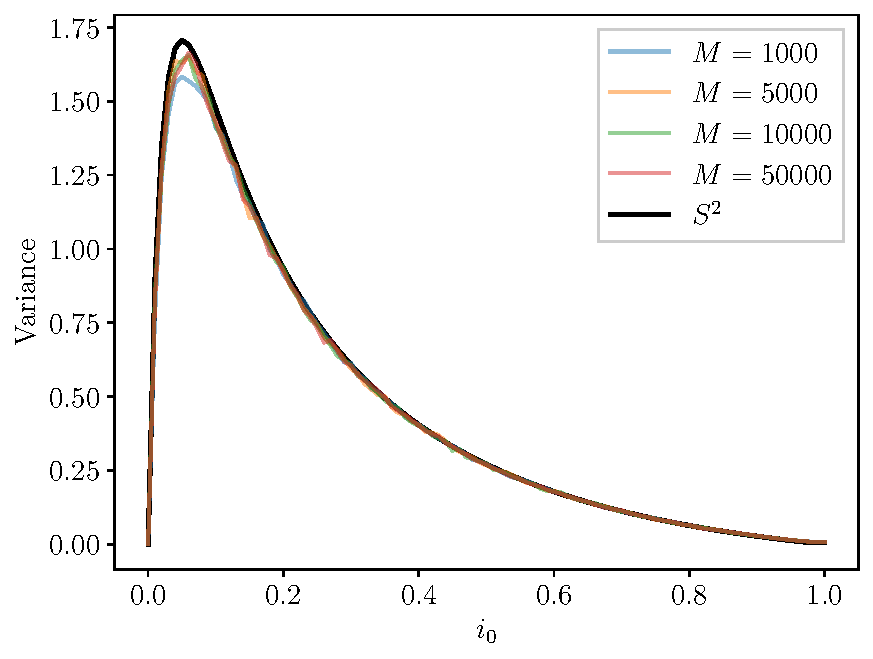
\includegraphics[width=\textwidth]{chp06_applications/figures/sir/sir_s2_1.0_1.0.pdf}
% 		% 	\caption{\(\beta = 1\), \(\gamma = 1\) (\(R_0 = 1\))}
% 		% \end{subfigure}
% 		% \begin{subfigure}{0.49\textwidth}
% 		% 	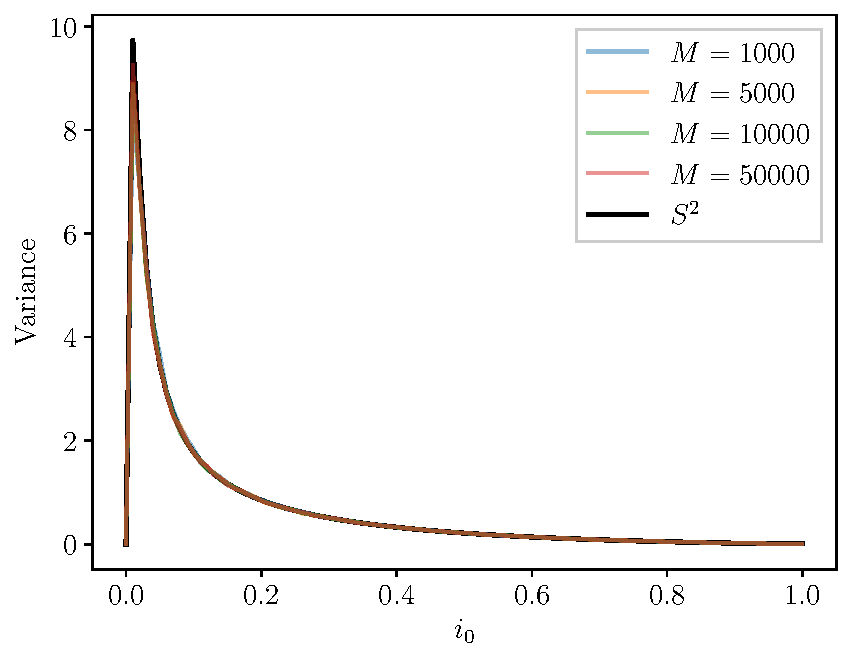
\includegraphics[width=\textwidth]{chp06_applications/figures/sir/sir_s2_1.5_1.0.pdf}
% 		% 	\caption{\(\beta = 1.5\), \(\gamma = 1\) (\(R_0 = 1.5\))}
% 		% \end{subfigure}\begin{subfigure}{0.49\textwidth}
% 		% 	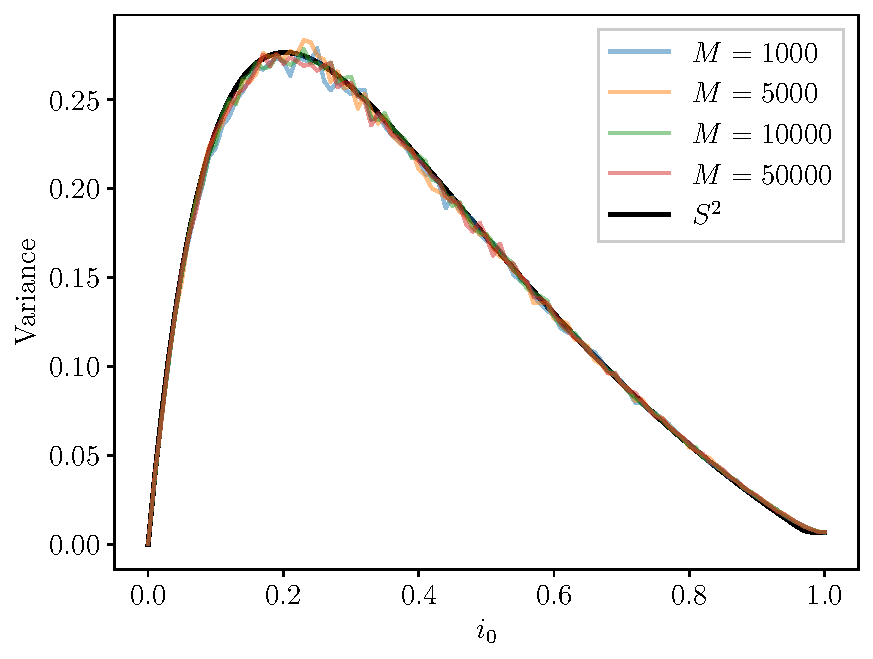
\includegraphics[width=\textwidth]{chp06_applications/figures/sir/sir_s2_0.5_1.0.pdf}
% 		% 	\caption{\(\beta = 0.5\), \(\gamma = 1\) (\(R_0 = 0.5\))}
% 		% \end{subfigure}
% 		% \begin{subfigure}{0.49\textwidth}
% 		% 			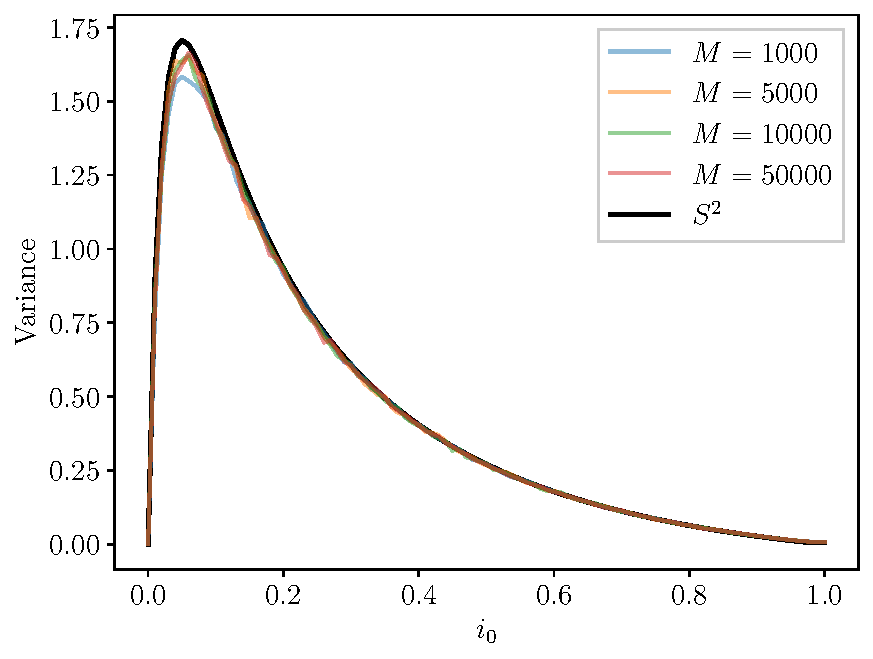
\includegraphics[width=\textwidth]{chp06_applications/figures/sir/sir_s2_1.0_1.0.pdf}
% 		% 			\caption{\(\beta = 2.0\), \(\gamma = 1\) (\(R_0 = 1\))}
% 		% 		\end{subfigure}
% 		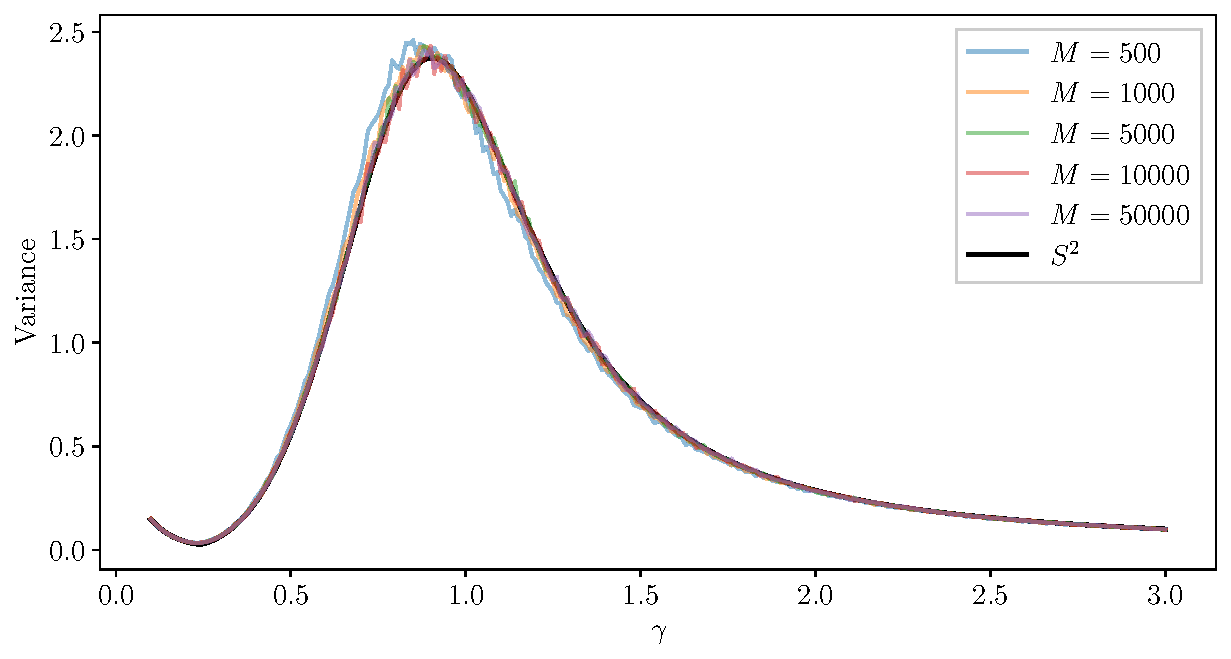
\includegraphics[width=\textwidth]{chp06_applications/figures/sir/sir_s2_R0}
% 		\caption{The stochastic sensitivity value (in black) of the SIR diffusion limit \cref{eqn:sir_diff_limit} at time \(T = 5\) and from the fixed initial proportion \(i_0 = 0.1\), for varying reproductive number \(R_0 = \beta / \gamma\).
% 			The maximum projection of the sample covariance matrix (in various colours) for \(N = 1000\) stochastic simulations of the discrete population process over the same time interval is included.
% 			The corresponding initial condition is \(\left(0.9M, 0.1M\right)^{\T}\)}
% 		\label{fig:sir_s2}
% 	\end{center}
% \end{figure}

% The limiting diffusion matrix provides a measure of how much variation is left unexplained when using the deterministic fluid limit \citep{PollettEtAl_2010_ModellingPopulationProcesses}, and is consistent with the stochastic sensitivity framework
% \td{Any interpretation when we ignore the population size?? Could be onto something here.}
% % The point of \Cref{fig:sir_s2} is that for \emph{any}



% \subsection{Example 2: Ebola model with 6 compartments}\label{sec:epi_5d}
% For our final example, we take a 6-compartment population process model that was used by \citet{LegrandEtAl_2007_UnderstandingDynamicsEbola} to analyse outbreaks of Ebola in the Democratic Republic of Congo in 1995 and in Uganda in 2000.


% For a fixed population size, this model is 5-dimensional.

% \begin{landscape}
% 	\begin{figure}
% 		\begin{center}
% 			\begin{tabular}{|c|c|c|c|}
% 				\hline
% 				Transition & \multicolumn{2}{c|}{Event}    & Rate \(\lambda_i\)                                                                                                     \\ \hline
% 				(1)        & Exposure                      & \(\left(S, E\right) \to \left(S-1, E+1\right)\)     & \(\left(\beta_I SI + \beta_H SH + \beta_F SF\right) / N\)        \\ \hline
% 				(2)        & Shedding                      & \(\left(E, I\right) \to \left(E - 1, I + 1\right)\) & \(\alpha E\)                                                     \\ \hline
% 				(3)        & Hospitalisation               & \(\left(I, H\right) \to \left(I - 1, H + 1\right)\) & \(\gamma_H \theta_1 I\)                                          \\ \hline
% 				(4)        & Hospital death without burial & \(\left(H, D\right) \to (H - 1, D + 1)\)            & \(\gamma_{dh}\delta_2 H\)                                        \\ \hline
% 				(5)        & Burial                        & \(\left(D\right) \to \left(D - 1\right)\)           & \(\gamma_f D\)                                                   \\ \hline
% 				(6)        & Death with burial             & \(\left(I\right) \to \left(I - 1\right)\)           & \(\gamma_i\left(1 - \theta_1\right)\left(1 - \delta_1\right) I\) \\ \hline
% 				(7)        & Death without burial          & \(\left(I, D\right) \to \left(I - 1, D + 1\right)\) & \(\delta_1 \left(1 - \theta_1\right) \gamma_d I\)                \\ \hline
% 				(8)        & Hospital death with burial    & \(\left(H\right) \to \left(H - 1\right)\)           & \(\gamma_{ih}\left(1 - \delta_2\right)H\)                        \\ \hline
% 			\end{tabular}

% 			\begin{tikzpicture}
% 				\node (S) [draw] {S};
% 				\node (E) [draw, right=of S] {E};
% 				\node (I) [draw, right=of E] {I};
% 				\node (H) [draw, right=of I] {H};
% 				\node (F) [draw, right=of H] {F};
% 				\node (R) [draw, right=of F] {R};
% 				\path[->,thick] (S) edge[above] node{(1)}  (E)
% 				(E) edge[above] node{(2)} (I)
% 				(I) edge[above] node{(3)} (H)
% 				(H) edge[above] node{(4)} (F)
% 				(F) edge[above] node{(5)} (R)
% 				(I) edge[bend right, below] node{(6)} (R)
% 				(I) edge[bend right, below] node{(7)} (F)
% 				(H) edge[bend left, above] node{(8)} (R);
% 			\end{tikzpicture}
% 			\caption{Transition probabilities of the Ebola model.}
% 			\label{fig:ebola_transition}
% 		\end{center}
% 	\end{figure}
% \end{landscape}


% The model consists of 6 compartments, so that an individual is one of:
% \begin{itemize}
% 	\item susceptible (\(S\)), having not yet been exposed to the virus,
% 	\item exposed (\(E\)), having been exposed to the virus but not yet infectious,
% 	\item infected (\(I\)), infected with the virus and infectious to susceptible individuals,
% 	\item hospitalised (\(H\)), infected with the virus but hospitalised,
% 	\item deceased (\(F\)) without burial, meaning that the individual is still infectious, and
% 	\item removed (\(R\)), meaning that the individual is no longer infectious or susceptible.
% \end{itemize}
% \Cref{fig:ebola_transition} shows the transition diagram and corresponding transitions rates between the compartments.


% \begin{landscape}
% 	\begin{figure}
% 		\begin{center}
% 			\begin{tabular}{|c|c|c|}
% 				\hline
% 				Parameter                                                               & Value               & Source                                                                                                                                 \\ \hline
% 				Population size \(M\)                                                   & 200000              & \citet{DowellEtAl_1999_TransmissionEbolaHemorrhagic}                                                                                   \\
% 				Initial cases \(I_0\)                                                   & 3                   & \citet{KhanEtAl_1999_ReemergenceEbolaHemorrhagic}                                                                                      \\
% 				Mean duration of incubation	\(\alpha\)                                  & \(1 / 7\) per day   & \citet{DowellEtAl_1999_TransmissionEbolaHemorrhagic,BwakaEtAl_1999_EbolaHemorrhagicFever,NdambiEtAl_1999_EpidemiologicClinicalAspects} \\
% 				Mean time to hospitalisation \(\gamma_h\)                               & \(1 / 9.6\) per day & \citet{KhanEtAl_1999_ReemergenceEbolaHemorrhagic}                                                                                      \\
% 				Mean duration of infectious period \(\gamma_i\)                         & \(1 / 10\) per day  & \citet{DowellEtAl_1999_TransmissionEbolaHemorrhagic,RoweEtAl_1999_ClinicalVirologicImmunologic}                                        \\
% 				Mean time to death \(\gamma_d\)                                         & \(1 / 2\) per day   & \citet{KhanEtAl_1999_ReemergenceEbolaHemorrhagic}                                                                                      \\
% 				Proportion of hospitalised cases \(\theta_1\)                           & \(0.67\)            & \citet{KhanEtAl_1999_ReemergenceEbolaHemorrhagic}                                                                                      \\
% 				Unhospitalised Case-fatality ratio (with burial) \(\delta_1\)           & \(0.8\)             & \citet{KhanEtAl_1999_ReemergenceEbolaHemorrhagic}                                                                                      \\
% 				Hospitalised case-fatality ratio (with burial)\(\delta_2\)              & \(0.8\)             & \citet{KhanEtAl_1999_ReemergenceEbolaHemorrhagic}                                                                                      \\
% 				Transmission rate in the community \(\beta_I\)                          & \(0.588\) per week  & \citet{LegrandEtAl_2007_UnderstandingDynamicsEbola}                                                                                    \\
% 				Transmission rate at the hospital \(\beta_H\)                           & \(0.794\) per week  & \citet{LegrandEtAl_2007_UnderstandingDynamicsEbola}                                                                                    \\
% 				Transmission rate during funerals \(\beta_F\)                           & \(7.653\) per week  & \citet{LegrandEtAl_2007_UnderstandingDynamicsEbola}                                                                                    \\
% 				Mean time from hospitalisation to death \(\gamma_{dh}\)                 & per week            & \citet{LegrandEtAl_2007_UnderstandingDynamicsEbola}                                                                                    \\
% 				Mean time from hospitalisation to end of infectiousness \(\gamma_{ih}\) & per week            & \citet{LegrandEtAl_2007_UnderstandingDynamicsEbola}                                                                                    \\
% 				\hline
% 			\end{tabular}
% 		\end{center}
% 		\caption{Parameter values for the Ebola model, estimated from the 1995 outbreak in the Democratic Republic of Congo.
% 			This table is adapted from Tables 3 and 4 of \citet{LegrandEtAl_2007_UnderstandingDynamicsEbola}, where values sourced directly from \citet{LegrandEtAl_2007_UnderstandingDynamicsEbola} have been estimated from morbidity data.}
% 		\td{Descriptions of variables not quite right}
% 		\label{tab:ebola_param_vals}
% 	\end{figure}
% \end{landscape}

% \Cref{tab:ebola_param_vals} provides parameter values for the model, including the physical interpretations of each parameter.
% These parameter values are taken from a combination of previous studies \citep{DowellEtAl_1999_TransmissionEbolaHemorrhagic,KhanEtAl_1999_ReemergenceEbolaHemorrhagic,BwakaEtAl_1999_EbolaHemorrhagicFever,NdambiEtAl_1999_EpidemiologicClinicalAspects} and estimates provided by \citet{LegrandEtAl_2007_UnderstandingDynamicsEbola}.
% The estimates of \citet{LegrandEtAl_2007_UnderstandingDynamicsEbola} are maximum likelihood estimates fitted on morbidity data from the 1995 Ebola outbreak in the Democratic Republic of Congo.


% Let \(X_t^{(N)} = \left(S_t / N, I_t / N, E_t / N, H_t / N, D_t / N\right)^{\T}\) denote the proportion of individuals in each compartment after \(t\) weeks.
% The population process is also density dependent, with
% \[
% 	f\!\left(\left(s, e, i, h, d\right), l\right) = \begin{cases}
% 		\beta_I s i + \beta_H sh + \beta_F sd,                        & \text{if } l = \left(-1, 1, 0, 0, 0\right), \\
% 		\alpha e,                                                     & \text{if } l = \left(0, -1, 1, 0, 0\right), \\
% 		\gamma_h \theta_1 i,                                          & \text{if } l = \left(0, 0, -1, 1, 0\right), \\
% 		\gamma_{dh}\delta_2 h,                                        & \text{if } l = \left(0, 0, 0, -1, 1\right), \\
% 		\gamma_f d,                                                   & \text{if } l = \left(0, 0, 0, 0, -1\right), \\
% 		\gamma_i\left(1 - \theta_1\right)\left(1 - \delta_1\right) i, & \text{if } l = \left(0,0,-1,0,0\right),     \\
% 		\delta_1\left(1 - \theta_1\right)\gamma_d i,                  & \text{if } l = \left(0,0,-1,0,1\right),     \\
% 		\gamma_{ih}\left(1 - \delta_2\right)h,                        & \text{if } l = \left(0,0,0,-1,0\right),     \\
% 		0,                                                            & \text{otherwise}.
% 	\end{cases}
% \]
% The deterministic differential equation is
% \[
% 	\dod{X_t^{(\infty)}}{t} = \begin{bmatrix}
% 		-\beta_I X_t^{(\infty, 1)}X_t^{(\infty, 3)} - \beta_H X_t^{(\infty, 1)}X_t^{(\infty, 4)} - \beta_F X_t^{(\infty, 1)}X_t^{(\infty,5)}                                                \\
% 		\beta_I X_t^{(\infty, 1)}X_t^{(\infty, 3)} + \beta_H X_t^{(\infty, 1)}X_t^{(\infty, 4)} + \beta_F X_t^{(\infty, 1)}X_t^{(\infty,5)} - \alpha X_t^{(\infty, 2)}                      \\
% 		\alpha X_t^{(\infty, 2)} - \left(\gamma_h\theta_1 + \gamma_i\left(1 - \theta_1\right)\left(1 - \delta_1\right) + \delta_1\left(1 - \theta_1\right)\gamma_d\right) X_t^{(\infty, 3)} \\
% 		\gamma_h\theta_1 X_t^{(\infty, 3)} - \left(\gamma_{dh}\delta_2 + \gamma_{ih}\left(1 - \delta_2\right) \right) X_t^{(\infty, 4)}                                                     \\
% 		\gamma_{dh}\delta_2 X_t^{(\infty, 4)} + \delta_1\left(1 - \theta_1\right)\gamma_d X_t^{(\infty, 3)} - \gamma_f X_t^{(\infty, 5)}
% 	\end{bmatrix}.
% \]
% The \(5\times 5\) diffusion matrix \(g\) satisfies

% \begin{scriptaligned}
% 	\left[g\!\left(X_t^{(\infty)}\right)g\!\left(X_t^{(\infty)}\right)^{\T}\right]_{11} & =	\beta_I X_t^{(\infty, 1)} X_t^{(\infty, 3)} + \beta_H X_t^{(\infty, 1)} X_t^{(\infty, 4)} + \beta_F X_t^{(\infty, 1)} X_t^{(\infty, 5)} \\
% 	\left[g\!\left(X_t^{(\infty)}\right)g\!\left(X_t^{(\infty)}\right)^{\T}\right]_{12} & = \left[g\!\left(X_t^{(\infty)}\right)g\!\left(X_t^{(\infty)}\right)^{\T}\right]_{21} =  -\beta_I X_t^{(\infty, 1)} X_t^{(\infty, 3)} - \beta_H X_t^{(\infty, 1)} X_t^{(\infty, 4)} - \beta_F X_t^{(\infty, 1)} X_t^{(\infty, 5)} \\
% 	\left[g\!\left(X_t^{(\infty)}\right)g\!\left(X_t^{(\infty)}\right)^{\T}\right]_{22} & = \beta_I X_t^{(\infty, 1)} X_t^{(\infty, 3)} + \beta_H X_t^{(\infty, 1)} X_t^{(\infty, 4)} + \beta_F X_t^{(\infty, 1)} X_t^{(\infty, 5)} +  \alpha X_t^{(\infty, 2)} \\
% 	\left[g\!\left(X_t^{(\infty)}\right)g\!\left(X_t^{(\infty)}\right)^{\T}\right]_{23} & = \left[g\!\left(X_t^{(\infty)}\right)g\!\left(X_t^{(\infty)}\right)^{\T}\right]_{32} = -\alpha X_t^{(\infty, 2)} \\
% 	\left[g\!\left(X_t^{(\infty)}\right)g\!\left(X_t^{(\infty)}\right)^{\T}\right]_{33} & = \alpha X_t^{(\infty, 2)} + \left(\gamma_H \theta_1  + \gamma_i(	1 - \theta_1)(1 - \delta_1) + \delta_1(1 - \theta_1)\gamma_d\right)X_t^{(\infty, 1)} \\
% 	\left[g\!\left(X_t^{(\infty)}\right)g\!\left(X_t^{(\infty)}\right)^{\T}\right]_{34} & = \left[g\!\left(X_t^{(\infty)}\right)g\!\left(X_t^{(\infty)}\right)^{\T}\right]_{43} = - \gamma_H \theta_1 X_t^{(\infty, 1)}\\
% 	\left[g\!\left(X_t^{(\infty)}\right)g\!\left(X_t^{(\infty)}\right)^{\T}\right]_{35} & = \left[g\!\left(X_t^{(\infty)}\right)g\!\left(X_t^{(\infty)}\right)^{\T}\right]_{53} = - \delta_1(1 - \theta_1)\gamma_d X_t^{(\infty, 1)}\\
% 	\left[g\!\left(X_t^{(\infty)}\right)g\!\left(X_t^{(\infty)}\right)^{\T}\right]_{44} & = \gamma_H \theta_1 X_t^{(\infty, 1)} + \left(\gamma_{dh}\delta_2  + \gamma_{ih}(1 - \delta_2)\right)X_t^{(\infty, 4)} \\
% 	\left[g\!\left(X_t^{(\infty)}\right)g\!\left(X_t^{(\infty)}\right)^{\T}\right]_{45} & = \left[g\!\left(X_t^{(\infty)}\right)g\!\left(X_t^{(\infty)}\right)^{\T}\right]_{54} = -\gamma_{dh}\delta_2 X_t^{(\infty, 4)} \\
% 	\left[g\!\left(X_t^{(\infty)}\right)g\!\left(X_t^{(\infty)}\right)^{\T}\right]_{55} & = \delta_1(1 - \theta_1)\gamma_d X_t^{(\infty, 1)} + \gamma_{dh}\delta_2 X_t^{(\infty, 4)} + \gamma_f X_t^{(\infty, 5)}
% \end{scriptaligned}
% with all other entries zero.
% There are many choices of \(g\) such that the product \(gg^{\T}\) has these entries, but to compute the Gaussian approximation with Mazzoni's method, we only need to evaluate \(g\!\left(X_t^{(\infty)}\right)g\!\left(X_t^{(\infty)}\right)\) and therefore no not need to make such a choice.





% \begin{landscape}
% 	\begin{figure}
% 		\centering
% 		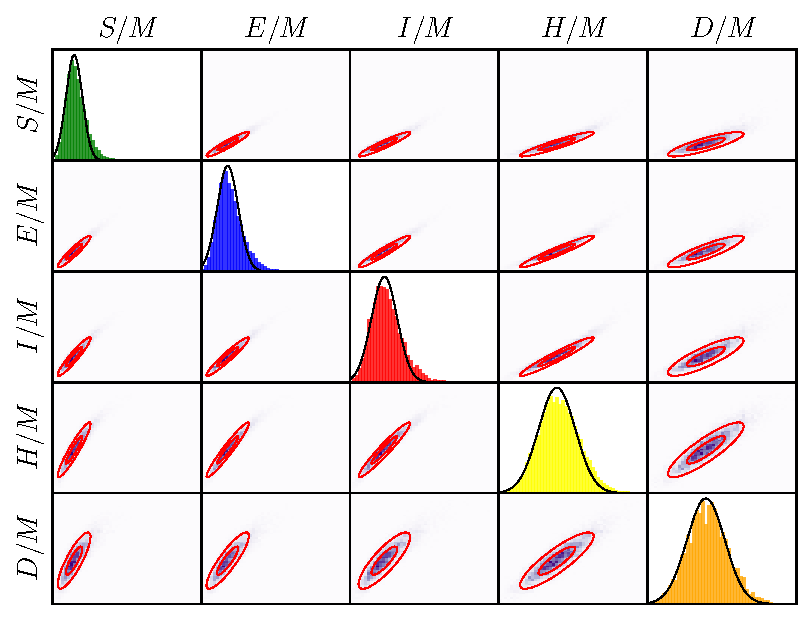
\includegraphics[width=\textheight]{chp06_applications/figures/seihfr/seihfr_marginals_gaussian}
% 		\caption{big guy}
% 		\label{fig:}
% 	\end{figure}
% \end{landscape}




% \begin{figure}
% 	\begin{center}
% 		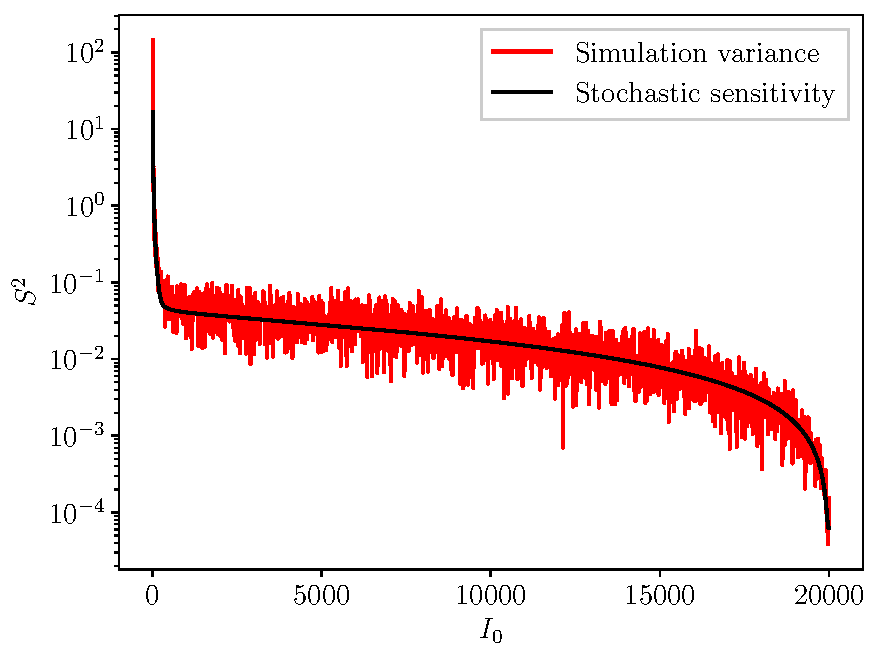
\includegraphics[width=\textwidth]{chp06_applications/figures/seihfr/seihfr_s2}
% 		\caption{}
% 		\label{fig:}
% 	\end{center}
% \end{figure}
